\documentclass[11pt,oneside]{uhthesis}
\usepackage{mathpazo}
\usepackage{amsmath}
\usepackage{tikz}
\usepackage{graphicx}
\usepackage{adjustbox}
\usetikzlibrary{positioning}
\usetikzlibrary{automata}
\usetikzlibrary{babel}

\renewcommand{\tablename}{Tabla}
\title{Una propuesta para encontrar el sistema de ecuaciones diferenciales lineales en los parámetros que mejor ajuste un conjunto de datos}
\author{Enrique Martínez González}
\advisor{MSc. Fernando Rodríguez Flores}
\coadvisor{Lic. Ernesto Borrego Rodríguez}
\degree{Licenciado en Ciencias de la Computación}
\faculty{Facultad de Matemática y Computación}
\date{Diciembre de 2022}
\logo{Graphics/uhlogo}


\begin{document}
\selectlanguage{spanish}

\frontmatter
\maketitle

\begin{dedication}
    \textit{
        A mi hermano,\\
        a mi madre,\\
        a mi padre,\\
        a mis abuelos,\\
        a mis amigos.
    }
\end{dedication}
\chapter*{Agradecimientos}\label{chapter:agradecimientos}

Un agradecimiento especial a que solo se fue la luz 2 veces

\begin{opinion}
    Y aqui va la opinión del tutor :D

    \vspace{1cm}


    \begin{flushright}
        \underline{\hspace{6.5cm}}\\
        MSc. Fernando Raul Rodriguez Flores

        Facultad de Matemática y Computación

        Universidad de la Habana

        Diciembre, 2022
    \end{flushright}

\end{opinion}
\begin{abstract}

    Resumen en español

\end{abstract}

\begin{enabstract}

    Abstract en inglés

\end{enabstract}
\include{FrontMatter/Contents}

\mainmatter

\chapter*{Introducción}\label{chapter:introduction}
\addcontentsline{toc}{chapter}{Introducción}

\qquad

Tengo que ver que pongo aqui de regresión porque todo lo moví para los preliminares
% La regresión es un conjunto de procesos estadísticos para estimar las relaciones entre una o más variables dependientes y una o más variables independientes \cite{johnson2015applied}. La variable dependiente es la que es explicada mientras que la independiente es la que se utiliza para explicar la variación de la variable independiente. Se le llama regresión simple si solo se tienen dos variables, una dependiente y una independiente, en caso de que se posean más variables independiente se le llama regresión múltiple. Si como resultado de la regresión se obtiene un hiperplano entonces obtiene el nombre de regresión lineal \cite{mann2007introductory}. Por ejemplo, el método de los mínimos cuadrados ordinarios calcula el único hiperplano que minimiza la suma de las diferencias al cuadrado entre los datos dados y ese hiperplano, este es un tipo de regresión. Este método se puede expresar como encontrar los valores de $\beta$ que minizan $S$ dado el modelo $f$ y los puntos $(xi, yi)$ donde:

% $$S = \sum_{i=1}^{n}(y_i - f(x_i, \beta))^2$$

% Teniendo este hiperplano, el investigador puede estimar la variable dependiente cuando las variables independientes toman un conjunto dado de valores.

% El análisis de regresión se puede utilizar para la predicción y el pronóstico de datos y en algunas situaciones, se puede utilizar el análisis de regresión para inferir relaciones causales entre las variables independientes y dependientes \cite{mann2007introductory}.

Teniendo en cuenta que la regresión permite encontrar los valores que mejor ajustan un modelo dado conjunto de datos, se puede intentar utilizar la regresión para determinar de forma automática el sistema de ecuaciones diferenciales ordinarias lineal en los parámetros que mejor describe un conjunto de puntos de la forma $(t_i, y_i)$.

Una función es lineal en los parámetros si es de la forma:

$$f(t,y) = \sum_{i=1}^{n} a_i * g_i(t, y)$$

donde los $a_i$ son parámetros y todas las funciones $g_i(t,y)$ son funciones que dependen de la variable $t$, de la variable $y$, pero no dependen de ningún parámetro.

Esta definición se puede extender a sistemas de ecuaciones si todas las funciones cumplen esta propiedad.

Un ejemplo de una función lineal con respecto a los parámetros sería:

\begin{equation}
    \label{eqn:ode_example}
    I` = a * I^2
\end{equation}

Si se plantea que $y(t_i)$ es la solución de la ecuación diferencial evaluada en el punto $t_i$, entonces un indicador de cuán bien el sistema describe los valores de $(ti, yi)$ pudiera ser el valor $L$, donde:

$$L = \sum_{i=1}^{n} (y(t_i) - y_i)^2$$

Cuando se usa un valor como $L$ en el que se considera la suma de cuadrados de las diferencias, se dice que estamos en presencia de un problema de mínimos cuadrados, porque lo que se quiere es minimizar esa suma de cuadrados.

Entonces, buscar el sistema de ecuaciones diferenciales que mejor describe los datos, se reduce a buscar el sistema de ecuaciones diferenciales que haga que el valor de $L$ sea lo más pequeño posible.

\subsection*{Objetivos}

El objetivo general de este trabajo es diseñar e implementar una herramienta que permita encontrar, con muy poco esfuerzo del usuario, el sistema de ecuaciones diferenciales lineales en los parámetros que mejor ajuste un conjunto de datos de la forma $(ti, yi)$ con $1 < i < n$. Para ello, se trazaron los siguientes objetivos específicos:


\subsubsection*{Objetivos específicos}

\begin{enumerate}
    \item Enunciar las diferencias que plantea la regresión simbólica sobre el resto de regresiones existentes.
    \item Plantear qué son las metaheurísticas, específicamente los algoritmos genéticos.
    \item Evaluar la calidad de la herramienta implementada ante distintos modelos de ecuaciones diferenciales.
    \item Analizar los resultados obtenidos a través de un conjunto de métricas(AÚN NO SE CUÁLES MÉTRICAS VOY A UTILIZAR) y técnicas de visualización.
\end{enumerate}

\subsection*{Organización de la tesis}

Este documento está organizado en 4 capítulos que recogen las
distintas etapas por las que transitó la investigación.

En el capítulo 1 \textbf{Elementos de la regresión simbólica} se realiza una
introducción a los elementos y conceptos de esta área abordados a lo largo
del trabajo.

\chapter{Preliminares}\label{chapter:preliminaries}

En el capítulo anterior se definió el objetivo de este trabajo, para ello se plantearon los conceptos de sistema de ecuaciones diferenciales lineales en los parámetros y la relación que existe entre ajustar un conjunto de datos y el algoritmo de mínimos cuadrados.

En la sección 1.1 de este capítulo se plantea lo que es una ecuación diferencial, en la sección siguiente se define de forma más detallada qué es una ecuación diferencial con respecto a los parámetros. Una técnica importante que se utilizó para el desarrollo de este trabajo es la regresión, los detalles se pueden encontrar en la sección 1.3. Las características ajuste cuadrático y regresión simbólica aparecen en las dos secciones siguientes respectivamente. A continuación en el capítulo se puede ver cómo se utiliza la regresión simbólica directamente en un sistema de ecuaciones diferenciales. En la última sección de este capítulo se detalla qué es un algoritmo genético y se plantean ejemplos de situaciones en las que es útil esta metaheurística.

A continuación se plantea que es una ecuación diferencial y se muestra un ejemplo de esta.

\section{Ecuaciones diferenciales}

Una ecuación diferencial se define como una ecuación que contiene las derivadas de una o más variables dependientes, con respecto a una o más variables independientes \cite{gaucel2014learning}. Una ecuación diferencial ordinaria (EDO) es una que contiene derivadas en función de una sola variable (por ejemplo, el tiempo). La forma general de una ecuación diferencial ordinaria es:

$$y'(t)=f(t, y(t)) \qquad y(t_0) = y_0$$

donde $y(t)$ es una función y $y_0$ es una condición inicial.

La solución de una ecuación diferencial es una función que al ser sustituida en la ecuación diferencial hace que se satisfaga dicha ecuación. Si además la ecuación diferencial es ordinaria, continua en un intervalo cerrado y se tienen condiciones iniciales, entonces la solución de dicha ecuación diferencial existe y es única. \cite{coddington1955theory}

Un ejemplo de ecuación diferencial ordinaria es:

$$y' = \frac{x^2}{y^3}$$

en donde la solución sería:

$$y = \sqrt[4]{\frac{4x}{3} + 4c}$$


\section{Ecuaciones diferenciales lineales con respecto a los parámetros}

Una ecuación diferencial es lineal con respecto a los parámetro si es de la forma

$$\frac{dX_i}{dt} = \sum_{i=1}^{n} a_i * f_i(t, y(t))$$

donde los $a_i$ son parámetros y todas las funciones $f_i(t,y)$ son funciones que dependen de la variable $t$, de la variable $y$, pero no dependen de ningún parámetro $a_i$.

Esta definición se puede extender a sistemas de ecuaciones diferenciales si todas las ecuaciones cumplen esta propiedad. Que el sistema sea lineal con repecto a los paráemtros permite modelar múltiples sistemas dinámicos poblaciones como el sistema de lotka volterra:

$$X' = \alpha * X - \beta * X * Y$$
$$Y' = \delta * X * Y - \gamma * Y$$

Para encontrar estos sistemas se utilizan diversas técnicas ya que muchas veces solo se poseen muestras de algún fenómeno físico en concreto y no se conoce las ecuaciones que lo describen, una de estas técnicas es la regresión.

\section{Regresión}

La regresión es un conjunto de procesos estadísticos para estimar las relaciones entre una o más variables dependientes y una o más variables independientes \cite{johnson2015applied}. Se explica la variable dependiente mientras que la independiente es la que se utiliza para explicar la variación de la variable dependiente. Se le llama regresión simple si solo se tienen dos variables, una dependiente y una independiente, en caso de que se posean más variables independiente se le llama regresión múltiple \cite{mann2007introductory}.

El análisis de regresión se puede utilizar para la predicción y el pronóstico de datos y en algunas situaciones, se puede utilizar el análisis de regresión para inferir relaciones causales entre las variables independientes y dependientes \cite{mann2007introductory}.

La primera forma de regresión fue el método de mínimos cuadrados, que fue publicado por Legendre en 1805, y por Gauss en 1809. Legendre y Gauss aplicaron el método al problema de determinar, a partir de observaciones astronómicas, las órbitas de los cuerpos alrededor del Sol, en su mayoría cometas, pero también más tarde los planetas menores recién descubiertos.

\section{Ajuste mínimo cuadrático de datos}

El método de mínimos cuadrados es un tipo de regresión que se utiliza para aproximar la solución de modelos en los que se conoce la función pero no sus parámetros. También se puede ver como un algoritmo para aproximar la solución de sistemas sobredeterminados, estos sistemas son conjuntos de ecuaciones en los que hay más ecuaciones que incógnitas.

Este método funciona minimizando la suma de los cuadrados de la diferencia entre un valor observado y el valor ajustado proporcionado por la función. Se puede expresar como resolver el problema de optimización de encontrar los valores de $\beta$ que minimizan $S$ dado el modelo $f$ y los puntos $(xi, yi)$ donde:

$$S = \sum_{i=1}^{n}(y_i - f(x_i, \beta))^2$$

Teniendo estos parámetros, se puede estimar la variable dependiente cuando las variables independientes toman un conjunto dado de valores. Este método se utiliza cuando la función es conocida, pero hay ocasiones en la práctica en las que esto no ocurre, para encontrar la función se puede utilizar un método llamado regresión simbólica.

\section{Regresión simbólica}

La regresión simbólica se utiliza para encontrar dentro de un espacio de funciones el modelo que mejor se ajuste a un conjunto de datos planteados. En este método, ningún modelo en particular se utiliza como punto de partida para la búsqueda del modelo que se desea encontrar. En su lugar se generan expresiones aleatorias que se forman combinando operaciones matemáticas, funciones analíticas, constantes y variables.

La introducción de la regresión simbólica generalmente se atribuye a John R. Koza \cite{zelinka2005analytic}. Koza mostró que la regresión simbólica puede usarse para descubrir modelos mediante la codificacion de expresiones matemáticas como árboles computacionales. En tales árboles, los nodos internos representan funciones ($+$, $-$, $*$, etc) que se extraen de un conjunto predeterminado de posibilidades, y los nodos hojas representan variables o constantes ($x_1$, $x_2$, $\dots$, $-1$, $\pi$, etc). Los parámetros en estos modelos usualmente se calculaban en el propio algoritmo o cada cierto tiempo se resolvía un problema de optimización pero esto es costoso.

Al no requerir una especificación a priori de un modelo, la regresión simbólica no se ve afectada por el desconocimiento de la estructura del modelo. Este método intenta descubrir las relaciones presentes en el conjunto de datos. Para lograr este fin, se prueban múltiples modelos posibles evaluando su calidad con respecto a alguna métrica de interés, en lugar de imponer una estructura de modelo que se considere matemáticamente manejable desde una perspectiva humana.

Para evaluar que tan cercano está el modelo obtenido con respecto al modelo original se define una función de ajuste. Esta hace que los resultados obtenidos a lo largo de la regresión simbólica sean cada vez mejores ya que tiene en cuenta no solo las métricas de error (valores que definen cuan cerca están los resultados obtenidos a los resultados deseados), sino cualquier métrica que desee definir el usuario con el objetivo de obtener un resultado con características específicas, por ejemplo modelos más pequeños o con menor cantidad de parámetros. Esto facilita el análisis posterior de los resultados al permitir asociar en el modelo obtenido algunos parámetros a significados de la vida real, por ejemplo la cantidad de individuos que mueren en cada instante de tiempo en el sistema de lotka volterra.

La regresión simbólica tiene la desventaja de además de ser un problema NP-difícil \cite{virgolin2022symbolic}, tener un espacio de búsqueda mucho más grande que otros tipos de problemas de ajustes de datos. Por ejemplo, tanto en la regresión lineal como no lineal, el espacio de búsqueda es $R^m$ y en la regresión simbólica se pueden explorar todas las funciones que van de $R^m$ a $R^n$.

Sin embargo, esta característica de poseer un espacio de búsqueda tan grande también tiene ventajas ya que el resultado pueden ser múltiples modelos y su correspondientes conjuntos de parámetros. Examinar esta colección de modelos resultantes permite al usuario identificar una solución que se ajuste mejor a alguna características en particular. Por ejemplo que el modelo posea ecuaciones con poca cantidad de parámetros o que la diferencia entre los datos evaluados en el modelo y los datos originales sea menor que un error específico.


\section{Regresión simbólica para EDOs}

La regresión simbólica ha sido utilizada de diversas maneras para encontrar sistemas de ecuaciones diferenciales, por ejemplo en el año 2014, un grupo de investigadores utilizaron esta técnica para encontrar sistemas dinámicos, generando para cada ecuación del sistema un grupo de ecuaciones. Luego probaban distintas combinaciones de las ecuaciones de estos subconjuntos hasta encontrar una que satisfaciera las condiciones de su investigación \cite{gaucel2014learning}. En el año 2008 se utilizó la regresión simbólica junto con el algoritmo de mínimos cuadrados para encontrar el sistema de ecuaciones diferenciales lineales en los parametros que mejor ajustase un conjunto de datos \cite{iba2008inference}

ver donde pongo esto:

Para funciones matemáticas, se utilizan diversos métodos en la regresión simbólica, uno de ellos es la recombinación de ecuaciones usando algoritmos evolutivos y uno de estos puede ser un algoritmo genético.

\section{Algoritmos genéticos}

Un algoritmo genético es una metaheurística inspirada en el proceso natural de selección \cite{mitchell1998introduction}. Son utilizados fundamentalmente para generar soluciones de alta calidad en problemas de optimización y búsqueda. Es un método para pasar de una población de "cromosomas" (por ejemplo, cadenas de unos y ceros, o "bits") a una nueva población mediante el uso de una especie de "selección natural" junto con los operadores inspirados en la genética de cruce, mutación y selección. Cada cromosoma consta de "genes" (por ejemplo, bits).

Los algoritmos genéticos son cómodos para resolver problemas de optimizacióon de la forma $min f(x)$, donde $x$ pertenece a un conjunto $C$ dado. Se le llama solución a cualquier $x$ de $C$. En dependencia de la estructura de $C$, las soluciones pueden tener distintas formas, por ejemplo vectores de números reales como en los problemas de optimización tradicionales o puedes ser árboles como en el caso de la regresión simbólica.

La evolución generalmente comienza a partir de una población de individuos generados aleatoriamente y es un proceso iterativo, se le llama generación a la población en cada iteración. En cada generación se evalúa la aptitud, o lo que quiere decir, el valor de la función objetivo en el problema de optimización que se está resolviendo de cada individuo de la población.

Los individuos más aptos se seleccionan de manera aleatoria de la población actual y las propiedades de estos se modifican utilizando las operaciones de mutación y cruzamiento para formar una nueva población. Esta nueva población toma el lugar de la población origen formando así una nueva generación de soluciones candidatas que se utiliza luego en la siguiente iteración del algoritmo. Comúnmente, el algoritmo termina cuando se ha producido un número máximo de generaciones o se ha alcanzado un nivel de aptitud satisfactorio para la población, también se puede detener el algoritmo en otras situaciones, por ejemplo que se haya recorrido todo el espacio de búsqueda, pero esto es poco usual debido al tamaño tan grande que suele tener este espacio.

El tamaño de la población depende de la naturaleza del problema, por ejemplo si intentamos minimizar el valor de una función convexa bastará con una población con una pequeña cantidad de individuos. Normalmente las poblaciones contiene varios cientos o miles de posibles soluciones ya el espacio de búsqueda suele ser grande. Como se menciona anteriormente, la población inicial suele generarse aleatoriamente, lo que permite explorar toda la gama de posibles soluciones en el espacio de búsqueda. Ocasionalmente, las soluciones pueden iniciarse en áreas donde es probable que se encuentren soluciones óptimas, por ejemplo si se desea encontrar el mínimo de una función, se pueden generar soluciones iniciales en donde la pendiente de la función evaluada en estas soluciones sea $0$ ya que esto es una condición necesaria para ser mínimo.

Durante cada generación, se selecciona una parte de la población para generar nuevos individuos. Las soluciones se seleccionan a través de un proceso basado en la aptitud, donde las soluciones más adecuadas medidas por una función de aptitud, suelen tener más probabilidades de ser seleccionadas, a este proceso se le llama selección. Algunos métodos de selección califican la aptitud de cada solución y seleccionan preferentemente las mejores soluciones asignando una mayor probabilidad de ser escogidas a estas, otros métodos califican solo una muestra aleatoria de la población, ya que el primer proceso puede llevar mucho tiempo.

Para generar una población de soluciones de una generación a otra se parte de los individuos seleccionados, a través de una combinación de operadores genéticos: mutación y cruzamiento. La mutación realiza cambios aleatorios en algún sitio del individuo seleccionado, por ejemplo si el individuo es la cadena 00000100, este puede ser mutado en su segunda posición para obtener 01000100. El cruzamiento intercambia subpartes aleatorias de dos individuos, obteniendo dos nuevos cromosomas. Por ejemplo, las cadenas 10000100 y 11111111 puedes ser cruzadas a partir de su tercera posición en cada una para producir 10011111 y 10011111. Resaltar que existen operaciones de cruzamiento en la que solo se obtiene un nuevo individuo como resultado de la operación.

Estas operaciones de cruzamiento, mutación y selección finalmente dan como resultado la población de soluciones de la próxima generación que es diferente de la generación inicial. Generalmente, la aptitud promedio habrá aumentado con este procedimiento para la población, ya que solo los mejores organismos de la primera generación junto con una pequeña proporción de soluciones menos aptas son seleccionados para reproducción. Estas soluciones menos aptas aseguran la diversidad genética dentro del acervo de características de los padres y, por lo tanto, aseguran la diversidad de propiedades de la siguiente generación de cromosomas.

La opinión sobre la importancia del cruzamiento frente a la mutación está dividida. Existen referencias en \cite{fogel2006evolutionary} que respaldan la importancia de la búsqueda basada en mutaciones.

Con el fin de recorrer de maneras distintas el espacio de búsqueda, vale la pena ajustar parámetros como la probabilidad de mutación, la probabilidad de cruzamiento y el tamaño de la población para encontrar configuraciones adecuadas para la clase de problema en la que se trabaja, por ejemplo una tasa de mutación muy pequeña puede conducir a la deriva genética, que es que desaparecen por completo algunos genes y se fijan los más frecuentes en las siguientes generaciones, resultando en una disminución en la diversidad genética de la población. Una tasa de cruzamiento demasiado alta puede conducir a una convergencia prematura del algoritmo genético. Un tamaño de población proporcional al espacio de búsqueda asegura suficiente diversidad genética para el problema que se desea solucionar, pero puede conducir a que la ejecución del algoritmo tome más tiempo y realice más cómpuntos.

Este proceso de creación de nuevas generaciones se repite hasta que se alcanza una condición de parada. Las condiciones de parada comunes son:

\begin{itemize}
    \item Se encuentra una solución que satisface criterios definidos por el usuario, pueden ser una cantidad de ajuste mínimo, o haber alcanzado un modelo más corto.
    \item Se alcanza el número máximo fijado de generaciones.
    \item Se alcanza la cantidad de tiempo o cómputo máximo asignado
    \item La aptitud de la solución con la clasificación más alta está alcanzando o ha alcanzado un nivel tal que las iteraciones sucesivas ya no producen mejores resultados.
    \item Combinaciones de lo anterior.
\end{itemize}

En este capitulo se han definido conceptos fundamentales para la completa comprensión de la propuesta de solución que utiliza regresión simbólica mediante un algoritmo genético para la obtención de un sistema de ecuaciones lineales con respecto a los parámetros. Para usar un algoritmo genético es necesario entonces definir varios elementos:

\begin{itemize}
    \item Cuáles son las posibles soluciones
    \item Cómo aplicar un operador de cruzamiento
    \item Cómo aplicar un operador de mutación
    \item Cómo determinar cuán buena es una solución
    \item Cómo determinar qué soluciones pasan a las próximas generaciones
\end{itemize}

Estos se defininen en el próximo capítulo.

\chapter{Propuesta de solución}\label{chapter:solution_proposal}

En este capítulo se plantea una forma de obtener, a partir de un conjunto de datos, un sistema de ecuaciones diferenciales lineales en los parámetros que describa los datos observados. El sistema se obtiene mediante el uso de la regresión simbólica utilizando un algoritmo genético. Para determinar cuán bien un sistema de ecuaciones diferenciales describe al conjunto de datos, se resuelve un problema de mínimos cuadrados para estimar los parámetros.

La sección \ref{section:solution_representation} detalla cómo se puede representar un sistema de EDOs lineales en los parámetros mediante un árbol computacional. En \ref{section:solution_cost} se explica la función de ajuste que se tiene en cuenta en la regresión simbólica planteada. En las secciones \ref{section:mutation}, \ref{section:xcross} y \ref{section:selection} se detallan las operaciones necesarias para la aplicación de un algoritmo genético: la mutación, el cruzamiento y la selección, respectivamente. A continuación se describe cómo representar sistemas de ecuaciones linales mediante árboles computacionales.


\section{Representación de Sistemas de EDOs mediante árboles}\label{section:solution_representation}

A partir de datos de la forma $\{(t_i, y_i)\}$, se puede determinar la cantidad de ecuaciones que posee el sistema: una por cada dimensión que tenga el vector $y$. Por ejemplo, si cada elemento de los datos es de la forma:

$$(t_i, y_{1_i}, y_{2_i}, y_{3_i}),$$

entonces se tiene la certeza de que el sistema de ecuaciones diferenciales que se desea tiene tres ecuaciones, y que los sistemas de ecuaciones en el espacio de búsqueda del método deben tener la forma:

$$y_1' = f_1(t, y_1, y_2, y_3)$$
$$y_2' = f_2(t, y_1, y_2, y_3)$$
$$y_3' = f_3(t, y_1, y_2, y_3).$$

Conociendo que el sistema debe tener $n$ ecuaciones se puede afirmar que las soluciones candidatas a solución son una lista de $n$ elementos. La posición $i$ de la lista representa la función $f_i(t,y_1,y_2, \dots, y_n)$.

Por ejemplo, en el modelo poblacional SIR:

\begin{align*}
    S' & = - aIS    \\
    I' & = aIS - bI \\
    R' & = bI,
\end{align*}

se puede plantear que:

\begin{align*}
    S'(t) & = f_S(t, S, I, R)  \\
    I'(t) & = f_I(t, S, I, R)  \\
    R'(t) & = f_R(t, S, I, R).
\end{align*}

Este sistema se puede representar con la lista:

$$[f_S(t, S, I, R), f_I(t, S, I, R), f_R(t, S, I, R)]$$
$$= [-aIS, aIS - bI, bI].$$

Una expresión aritmética (como cada una de las posibles funciones) se puede representar mediante un árbol, donde los nodos interiores son operadores y las hojas son variables. Entonces en la posición $i$ de la lista, se puede representar el árbol computacional que describe la parte de la derecha de la ecuación diferencial correspondiente a la ecuación $i$.

Sin embargo, con la representación descrita por Koza \cite{zelinka2005analytic}, no se plantea de forma explícita la linealidad de las ecuaciones diferenciales con respecto a los parámetros, esta linealidad es importante dado que el sistema que se busca como solución debe cumplir esta propiedad. La representación planteada por Koza no resulta útil ya que en el algoritmo genético que se propone solo deben aparecer modelos que cumplan esta propiedad de linealidad. Para que la representación de las funciones en forma de árboles computacionales solo permita la linealidad con respecto a los parámetros, en este trabajo se modifica la estructura del árbol de la siguiente manera.

Como la parte derecha de una ecuación diferencial lineal con respecto a los parámetros es una suma de multiplicaciones de parámetros con funciones que no dependen de parámetros:

$$\frac{dX_i}{dt} = \sum_{i=1}^{n} a_i * f_i(t, y(t)),$$

entonces cada una de las partes derechas de las ecuaciones diferenciales se representan con un árbol en el que la raíz es un nodo con una operación especial de suma, que puede tener cualquier cantidad de sumandos (o de hijos) como se muestra en la figura \ref{tikzpicture:doe_node_example}.

% \begin{center}
%     \begin{tikzpicture}[
%             roundnode/.style={circle, draw, fill=gray!25, very thick, minimum size=7mm},
%             roundnode_transparent/.style={circle, very thick, minimum size=5mm}
%         ]
%         % Nodes
%         \node[roundnode]        (plus)                            {$+$};
%         \node[roundnode]        (term_1)     [below left=of plus]        {$a_1 * f_1(t, y(t))$};
%         \node[roundnode_transparent]        (term_dots)     [below =of plus]        {$\dots$};
%         \node[roundnode]        (term_n)     [below right=of plus]        {$a_n * f_n(t, y(t))$};


%         %Lines
%         \draw [->] (plus.south) -- (term_1.north);
%         % \draw [->] (plus.south) -- (term_dots.north);
%         \draw [->] (plus.south) -- (term_n.north);
%     \end{tikzpicture}
% \end{center}

\begin{figure}[h]
    \centering
    \includegraphics[width=0.5\textwidth]{"figures/doe_node_example.pdf"}
    \caption{Estructura del árbol de una ecuación diferencial lineal en los parámetros.}
    \label{tikzpicture:doe_node_example}
\end{figure}

Cada uno de los hijos del nodo que representa la parte derecha de una ecuación diferencial es un subárbol que representa la multiplicación de un parámetro con una función que no depende de parámetros.

Estos subárboles poseen como raíz un nodo con una operación de multiplicación y dos nodos hijos. El primero de ellos es un nodo hoja que representa el parámetro. El segundo hijo es un nodo que representa el subárbol computacional correspondiente a la función, utilizando la misma representación que plantea Koza \cite{zelinka2005analytic} pero con la peculiaridad de que sus hojas solo podrán almacenar variables, no parámetros como se muestra en la figura \ref{tikzpicture:doe_term_node_example}.

% \begin{center}
%     \begin{tikzpicture}[
%             roundnode/.style={circle, draw, fill=gray!25, very thick, minimum size=7mm},
%             squarednode/.style={rectangle, draw, fill=gray!25, very thick, minimum size=7mm}
%         ]
%         % Nodes
%         \node[roundnode]        (star)                            {$*$};
%         \node[squarednode]        (term_1)     [below left=of star]        {$a_i$};
%         \node[roundnode]        (term_n)     [below right=of star]        {$f_i(t, y(t))$};


%         %Lines
%         \draw [->] (star.south) -- (term_1.north);
%         \draw [->] (star.south) -- (term_n.north);
%     \end{tikzpicture}
% \end{center}

\begin{figure}[h]
    \centering
    \includegraphics[width=0.5\textwidth]{"figures/doe_term_node_example.pdf"}
    \caption{Estructura del árbol de un término perteneciente a una ecuación diferencial lineal en los parámetros.}
    \label{tikzpicture:doe_term_node_example}
\end{figure}


Un sistema de ecuaciones diferenciales se puede representar como un árbol donde cada ecuación sea un hijo. Como ejemplo se puede utilizar el modelo poblacional SIR, que es lineal con respecto a sus parámetros, y su representación con la estructura propuesta sería la figura \ref{tikzpicture:sir_example}.

% \begin{center}
%     \begin{tikzpicture}[
%             roundnode/.style={circle, draw, fill=gray!25, very thick, minimum size=7mm},
%             squarednode/.style={rectangle, draw, fill=gray!25, very thick, minimum size=5mm}
%         ]
%         % Nodes
%         \node[roundnode]        (system)                            {$SYSTEM$};

%         \node[roundnode]        (plus_S)     [below left=of system]        {$+$};
%         \node[roundnode]        (star_S_1)    [below left=of plus_S]    {$*$};
%         \node[squarednode]      (alpha_star_S_1)      [below left=of star_S_1]    {$a$};
%         \node[roundnode]        (neg_star_S_1)    [below=of star_S_1]    {$-$};
%         \node[roundnode]        (star_S_2)    [below=of neg_star_S_1]    {$*$};
%         \node[squarednode]      (S_star_S)       [below left=of star_S_2]   {$S$};
%         \node[squarednode]      (I_star_S)      [below=of star_S_2]   {$I$};

%         \node[roundnode]        (plus_I)     [below=of system]        {$+$};
%         \node[roundnode]        (star_I_1)    [below left=of plus_I]    {$*$};
%         \node[squarednode]      (alpha_star_I_1)      [below left=1cm and 0.5cm of star_I_1]    {$a$};
%         \node[roundnode]        (star_I_2)    [below=of star_I_1]    {$*$};
%         \node[squarednode]      (S_star_I)       [below left=1cm and 0.5cm of star_I_2]   {$S$};
%         \node[squarednode]      (I_star_I_1)      [below=of star_I_2]   {$I$};

%         \node[roundnode]        (star_I_3)    [below right=of plus_I]    {$*$};
%         \node[squarednode]      (beta_star_I_1)      [below=of star_I_3]    {$b$};
%         \node[roundnode]        (neg_star_I_1)    [below right=1cm and 0.5cm of star_I_3]    {$-$};
%         \node[squarednode]      (I_star_I_2)      [below=of neg_star_I_1]   {$I$};

%         \node[roundnode]        (plus_R)     [below right=of system]        {$+$};
%         \node[roundnode]        (star_R_1)    [below right=of plus_R]    {$*$};
%         \node[squarednode]      (beta_star_R_1)      [below=of star_R_1]    {$b$};
%         \node[squarednode]      (I_star_R)      [below right=of star_R_1]   {$I$};

%         %Lines
%         \draw [->] (system.south) -- (plus_S.north);
%         \draw[->] (system.south) -- (plus_I.north);
%         \draw[->] (system.south) -- (plus_R.north);

%         \draw[->] (plus_S.south) -- (star_S_1.north);
%         \draw[->] (star_S_1.south) -- (alpha_star_S_1.north);
%         \draw[->] (star_S_1.south) -- (neg_star_S_1.north);
%         \draw[->] (neg_star_S_1.south) -- (star_S_2.north);
%         \draw[->] (star_S_2.south) -- (S_star_S.north);
%         \draw[->] (star_S_2.south) -- (I_star_S.north);

%         \draw[->] (plus_I.south) -- (star_I_1.north);
%         \draw[->] (plus_I.south) -- (star_I_3.north);
%         \draw[->] (star_I_1.south) -- (alpha_star_I_1.north);
%         \draw[->] (star_I_1.south) -- (star_I_2.north);
%         \draw[->] (star_I_2.south) -- (S_star_I.north);
%         \draw[->] (star_I_2.south) -- (I_star_I_1.north);

%         \draw[->] (star_I_3.south) -- (beta_star_I_1.north);
%         \draw[->] (star_I_3.south) -- (neg_star_I_1.north);
%         \draw[->] (neg_star_I_1.south) -- (I_star_I_2.north);

%         \draw[->] (plus_R.south) -- (star_R_1.north);
%         \draw[->] (star_R_1.south) -- (beta_star_R_1.north);
%         \draw[->] (star_R_1.south) -- (I_star_R.north);
%     \end{tikzpicture}
% \end{center}

\begin{figure}[h]
    \centering
    \includegraphics[width=0.5\textwidth]{"figures/sir_example.pdf"}
    \caption{Estructura del árbol que representa el modelo poblacional SIR.}
    \label{tikzpicture:sir_example}
\end{figure}

Con esta representación se pueden expresar todos los sistemas de ecuaciones diferenciales lineales en los parámetros en los que intervengan un conjunto de operaciones prefijadas de antemano, que son los posibles nodos interiores. Esta representación se utiliza para la representación de los modelos que se generan en el algoritmo de regresión simbólica que se detalla en la secciones \ref{section:mutation} y \ref{section:xcross}.

En un método de regresión simbólica es necesaria una función de ajuste que permita conocer cuán cercanos son los datos predichos por el modelo con respecto a los datos observados. En la siguiente sección se propone un método para evaluar cuán cercanos se encuentran los datos predichos y observados.

\section{Determinar el costo de una solución}\label{section:solution_cost}

A partir de un conjunto de datos $M = \{(t_i, y_i)\}$ se puede aproximar el valor de las derivadas de $y_i$ en cada instante $t_i$ utilizando el método de diferencias finitas \cite{gaucel2014learning}. Con este método se puede generar un nuevo conjunto de la forma $\{(x_i, y'_i)\}$ donde $x_i \in M$ y $y'_i$ es el vector de las aproximaciones de los valores de las derivadas de las variables $y_i$ en el instante $t_i$.

Si $n$ es la cantidad de ecuaciones en el sistema y $m$ es la cantidad de datos, se define el costo de un sistema de ecuaciones diferenciales $f$ como:

$$C = \frac{\sum_{i=1}^n\frac{\sum_{j=1}^{m}(y'_{i_j} - f_i(x_j))^2}{m}}{n},$$

donde:

$$f_i(x_j) = \sum_{k=1}^{p_i} a_{i_k} * g_{i_k}(x_j),$$

y $f_1, f_2, \dots, f_n$ son las partes derechas de las ecuaciones del sistema y $p_i$ indica la cantidad de parámetros presentes en la ecuación $i$ del sistema. Mientras más pequeño es el valor del costo, mejor se describen los datos mediante el sistema f.

Al valor de $C$ se le agrega un factor de peso $P$, el cual es directamente proporcional a la cantidad de términos que posean las ecuaciones de la solución \cite{gplearnbloat}:

$$P = \begin{cases}
        Constant * node\_count(f), & \text{si } node\_count(f) \geq MAX\_NODES \\
        0,                         & \text{en otro caso}
    \end{cases}.$$

$node\_count(f)$ es la cantidad de nodos presentes en la representación en forma de árbol computacional del sistema $f$. $Constant$ es una constante definida en la implementación, en los experimentos realizados en el capítulo \ref{chapter:results} se utiliza un valor de 9999.

El parámetro $MAX\_NODES$ se define junto con los demás parámetros del algoritmo genético. El factor de peso garantiza que si dos ecuaciones son capaces de generar los mismos puntos, la ecuación con menos términos tenga una mejor evaluación en la función objetivo.

Para que la suma $\sum_{j=1}^{m}(y'_{i_j} - f_i(x_j)) ^ 2$ sea la menor posible se debe minimizar la diferencia $(y'_{i_j} - f_i(x_j))^2$. Para minimizar la diferencia se ajustan los parámetros $a_{i_k}$ presentes en cada una de las ecuaciones $f_i$. Es por ello que se crea, por cada ecuación del sistema, un sistema de ecuaciones de la forma $A_i * x_i = B_i$ donde:

\begin{align*}
    A_i & = \begin{pmatrix}
        g_{i_1}(x_1) & g_{i_2}(x_1) & \dots  & g_{i_k}(x_1) \\
        g_{i_1}(x_2) & g_{i_2}(x_2) &        & g_{i_k}(x_2) \\
        \vdots       & \vdots       & \ddots & \vdots       \\
        g_{i_1}(x_m) & g_{i_2}(x_m) &        & g_{i_k}(x_m)
    \end{pmatrix}
    \qquad
    x_i = \begin{bmatrix}
        a_{i_1} \\
        a_{i_2} \\
        \vdots  \\
        a_{i_k}
    \end{bmatrix}
    \qquad
    B_i = \begin{bmatrix}
        y'_{i_1} \\
        y'_{i_2} \\
        \vdots   \\
        y'_{i_m}
    \end{bmatrix}.
\end{align*}

El sistema $A_ix_i = B_i$ se resuelve utilizando el método de ajuste mínimo cuadrático de datos, descrito en el capítulo \ref{chapter:preliminaries}.

Por ejemplo, la segunda ecuación del modelo SIR es:

$$f_I (t,S,I,R) = a_{I_1} * g_{I_1}(t,S,I,R) + a_{I_2} * g_{I_2}(t,S,I,R),$$

donde:

$$g_{I_1}(t,S,I,R) = I*S$$

y

$$g_{I_2}(t,S,I,R) = -I.$$

Suponiendo que se tienen los puntos de la forma $\{(x_i, y'_i)\}$ donde $x_i$ es un vector representa los valores de $(t_i, S_i, I_i, R_i)$ y $y'_i$ es un vector que representa los valores de $(S_i', I_i', R_i')$:

\begin{align*}
    ((1, 4, 9, 6)  & ,  (0, 5, 0))  \\
    ((2, 6, 8, 2)  & ,  (0, 4, 0))  \\
    ((3, 3, 6, 8)  & ,  (0, 10, 0)) \\
    ((4, 5, 9, 8)  & ,  (0, 1, 0))  \\
    ((5, 6, 3, 10) & , (0, 7, 0))   \\
    ((6, 8, 5, 7)  & ,  (0, 6, 0)), \\
\end{align*}

entonces se puede encontrar los valores de $a_1$ y $a_2$ que mejor ajusten la ecuación con los puntos planteados anteriormente formando el sistema de ecuaciones:

\begin{align*}
    A_I & = \begin{pmatrix}
        36 & -9 \\
        48 & -8 \\
        18 & -6 \\
        45 & -9 \\
        18 & -3 \\
        40 & -5
    \end{pmatrix}
    \qquad
    x_I = \begin{bmatrix}
        a_{I_1} \\
        a_{I_2}
    \end{bmatrix}
    \qquad
    B_I = \begin{bmatrix}
        5  \\
        4  \\
        10 \\
        1  \\
        7  \\
        6
    \end{bmatrix}.
\end{align*}

Al resolver el sistema de ecuaciones sobredeterminado se obtienen los parámetros $a_{I_1}$ = -0.03570806 y $a_{I_2}$ = -0.84347764. El método de ajuste mínimo cuadrático de datos se aplica para encontrar los parámetros de cada una de las ecuaciones del sistema.

Como se mencionó al inicio del capítulo, la propuesta de solución utiliza el método de regresión simbólica mediante el uso de un algoritmo genético para encontrar el sistema que mejor ajuste un conjunto de puntos. Para usar el algoritmo genético es necesario definir las operaciones de mutación, cruzamiento y selección. En la siguiente sección se define la primera de las operaciones.

\section{Mutación}\label{section:mutation}

La operación de mutación genera un nuevo sistema de ecuaciones diferenciales modificando un sistema existente. Esta operación selecciona el subárbol representante de una de las ecuaciones en el sistema y luego se escoge una de las siguientes modificaciones:

\begin{itemize}
    \item Eliminar un término (sumando de la ecuación) de la ecuación. Si se toman los sumandos de la ecuación como una lista de términos, el criterio consiste en seleccionar un término y eliminarlo.

          Por ejemplo, si se tiene la ecuación

          $$a_1 * y_1 + a_2 * -(y_1 * y_2),$$

          la lista de términos correspondientes sería:

          $$[a_1*y_1, a_2 * -(y_1 * y_2)].$$

          Si se selecciona eliminar el segundo término, la ecuación resultante sería:

          $$a_1 * y_1.$$

          El ejemplo se puede expresar en forma de árbol computacional de la siguiente manera:

          \begin{center}
              \begin{adjustbox}{width=0.35\textwidth, keepaspectratio}
                  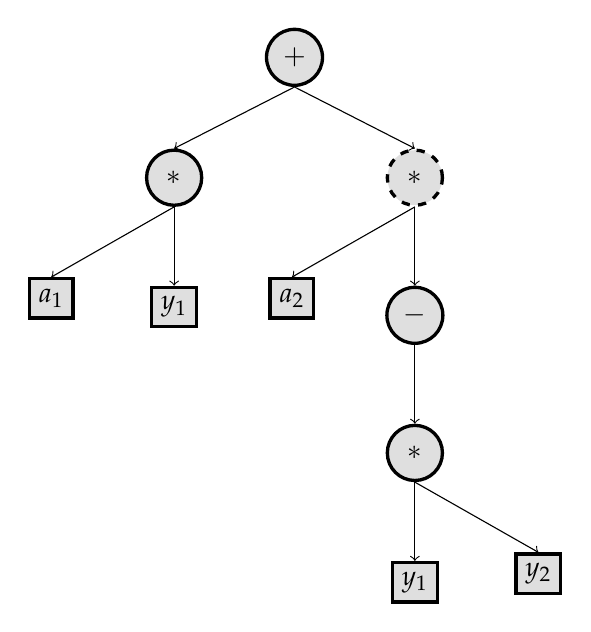
\begin{tikzpicture}[
                          roundnode_dashed/.style={circle, draw, dashed, fill=gray!25, very thick, minimum size=7mm},
                          roundnode/.style={circle, draw, fill=gray!25, very thick, minimum size=7mm},
                          squarednode/.style={rectangle, draw, fill=gray!25, very thick, minimum size=5mm},
                      ]
                      %Nodes
                      \node[roundnode]      (plus)                             {$+$};
                      \node[roundnode]           (star1)   [below left=of plus]    {$*$};
                      \node[squarednode]         (a_1)   [below left=of star1]    {$a_1$};
                      \node[squarednode]         (y_1)     [below=of star1]         {$y_1$};
                      \node[roundnode_dashed]           (star2)   [below right=of plus]   {$*$};
                      \node[squarednode]         (a_2)    [below left=of star2]    {$a_2$};
                      \node[roundnode]           (neg)     [below=of star2]         {$-$};
                      \node[roundnode]           (star3)   [below=of neg]         {$*$};
                      \node[squarednode]         (y_1_2)   [below=of star3]   {$y_1$};
                      \node[squarednode]         (y_2)     [below right=of star3]   {$y_2$};

                      %Lines
                      \draw[->] (plus.south) -- (star1.north);
                      \draw[->] (plus.south) -- (star2.north);
                      \draw[->] (star1.south) -- (a_1.north);
                      \draw[->] (star1.south) -- (y_1.north);
                      \draw[->] (star2.south) -- (a_2.north);
                      \draw[->] (star2.south) -- (neg.north);
                      \draw[->] (neg.south) -- (star3.north);
                      \draw[->] (star3.south) -- (y_1_2.north);
                      \draw[->] (star3.south) -- (y_2.north);
                  \end{tikzpicture}%
              \end{adjustbox}
              \qquad
              \begin{adjustbox}{width=0.20\textwidth, keepaspectratio}
                  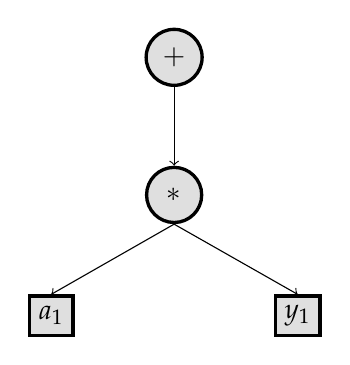
\begin{tikzpicture}[
                          roundnode_dashed/.style={circle, draw, dashed, fill=gray!25, very thick, minimum size=7mm},
                          roundnode/.style={circle, draw, fill=gray!25, very thick, minimum size=7mm},
                          squarednode/.style={rectangle, draw, fill=gray!25, very thick, minimum size=5mm},
                      ]
                      %Nodes
                      \node[roundnode]      (plus)                             {$+$};
                      \node[roundnode]           (star1)   [below =of plus]    {$*$};
                      \node[squarednode]         (a_1)   [below left=of star1]    {$a_1$};
                      \node[squarednode]         (y_1)     [below right=of star1]         {$y_1$};

                      %Lines
                      \draw[->] (plus.south) -- (star1.north);
                      \draw[->] (star1.south) -- (a_1.north);
                      \draw[->] (star1.south) -- (y_1.north);
                  \end{tikzpicture}%
              \end{adjustbox}
          \end{center}

    \item Añadir un término a la ecuación. Si se toman los sumandos de la ecuación como una lista de términos, el criterio consiste en crear un término y añadirlo.

          Por ejemplo, si se tiene la ecuación

          $$a_1 * y_1,$$

          la lista de términos correspondientes sería:

          $$[a_1*y_1].$$

          Si se selecciona añadir como segundo sumando el término $a_2 * y_2$, la ecuación resultante sería:

          $$a_1 * y_1 + a_2 * y_2.$$

          El ejemplo se puede expresar en forma de árbol computacional de la siguiente manera:

          \begin{center}
              \begin{adjustbox}{width=0.25\textwidth, keepaspectratio}
                  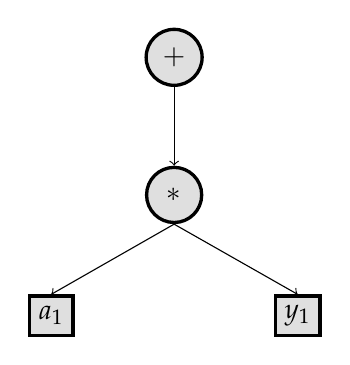
\begin{tikzpicture}[
                          roundnode_dashed/.style={circle, draw, dashed, fill=gray!25, very thick, minimum size=7mm},
                          roundnode/.style={circle, draw, fill=gray!25, very thick, minimum size=7mm},
                          squarednode/.style={rectangle, draw, fill=gray!25, very thick, minimum size=5mm},
                      ]
                      %Nodes
                      \node[roundnode]      (plus)                             {$+$};
                      \node[roundnode]           (star1)   [below =of plus]    {$*$};
                      \node[squarednode]         (a_1)   [below left=of star1]    {$a_1$};
                      \node[squarednode]         (y_1)     [below right=of star1]         {$y_1$};

                      %Lines
                      \draw[->] (plus.south) -- (star1.north);
                      \draw[->] (star1.south) -- (a_1.north);
                      \draw[->] (star1.south) -- (y_1.north);
                  \end{tikzpicture}%
              \end{adjustbox}
              \qquad
              \begin{adjustbox}{width=0.35\textwidth, keepaspectratio}
                  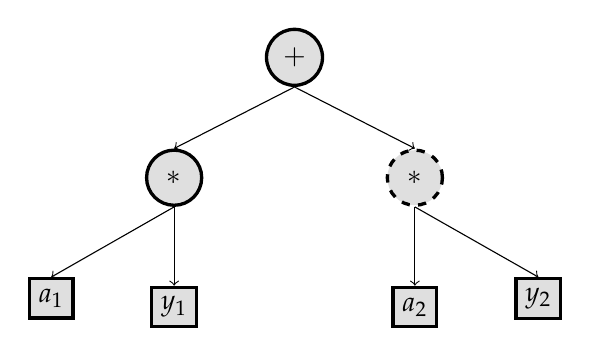
\begin{tikzpicture}[
                          roundnode_dashed/.style={circle, draw, dashed, fill=gray!25, very thick, minimum size=7mm},
                          roundnode/.style={circle, draw, fill=gray!25, very thick, minimum size=7mm},
                          squarednode/.style={rectangle, draw, fill=gray!25, very thick, minimum size=5mm},
                      ]
                      %Nodes
                      \node[roundnode]      (plus)                             {$+$};
                      \node[roundnode]           (star1)   [below left=of plus]    {$*$};
                      \node[squarednode]         (a_1)   [below left=of star1]    {$a_1$};
                      \node[squarednode]         (y_1)     [below=of star1]         {$y_1$};
                      \node[roundnode_dashed]           (star2)   [below right=of plus]   {$*$};
                      \node[squarednode]         (a_2)    [below=of star2]    {$a_2$};
                      \node[squarednode]           (y_2)     [below right=of star2]         {$y_2$};

                      %Lines
                      \draw[->] (plus.south) -- (star1.north);
                      \draw[->] (plus.south) -- (star2.north);
                      \draw[->] (star1.south) -- (a_1.north);
                      \draw[->] (star1.south) -- (y_1.north);
                      \draw[->] (star2.south) -- (a_2.north);
                      \draw[->] (star2.south) -- (y_2.north);
                  \end{tikzpicture}%
              \end{adjustbox}
          \end{center}

    \item Mutar un término de la ecuación. Si se toman los sumandos de la ecuación como una lista de términos, el criterio consiste en seleccionar un término y dentro de su representación en forma de árbol computacional, tomar un nodo y aplicarle una de las siguientes modificaciones.
\end{itemize}

Si el nodo representa una operación:

\begin{itemize}
    \item Se cambia la operación en el nodo por uno que posea la misma cantidad de argumentos del operador:

          Por ejempo, si se tiene el término $y_1 + (y_2 - y_3)$ se puede sustituir la resta por una suma resultando $y_1 + (y_2 + y_3)$. Si se expresa en forma de árbol computacional sería:

          \begin{center}
              \begin{adjustbox}{width=0.25\textwidth, keepaspectratio}
                  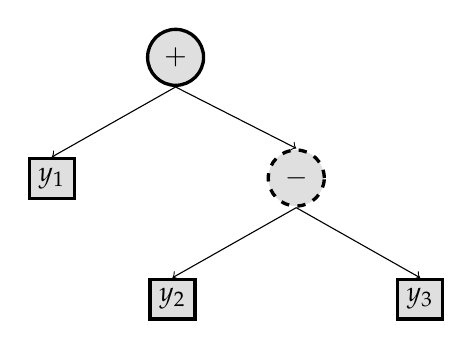
\begin{tikzpicture}[
                          roundnode_dashed/.style={circle, draw, dashed, fill=gray!25, very thick, minimum size=7mm},
                          roundnode/.style={circle, draw, fill=gray!25, very thick, minimum size=7mm},
                          squarednode/.style={rectangle, draw, fill=gray!25, very thick, minimum size=5mm},
                      ]
                      %               %Nodes
                      \node[roundnode]      (plus)                            {$+$};
                      \node[squarednode]    (y_1)     [below left=of plus]    {$y_1$};
                      \node[roundnode_dashed]      (sub)     [below right=of plus]   {$-$};
                      \node[squarednode]    (y_2)     [below left=of sub]     {$y_2$};
                      \node[squarednode]    (y_3)     [below right=of sub]    {$y_3$};


                      %   %Lines
                      \draw[->] (plus.south) -- (y_1.north);
                      \draw[->] (plus.south) -- (sub.north);
                      \draw[->] (sub.south) -- (y_2.north);
                      \draw[->] (sub.south) -- (y_3.north);
                  \end{tikzpicture}%
              \end{adjustbox}
              \qquad
              \begin{adjustbox}{width=0.25\textwidth, keepaspectratio}
                  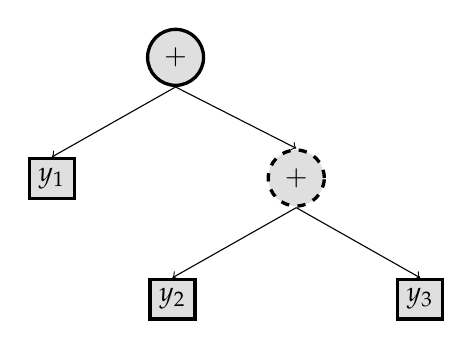
\begin{tikzpicture}[
                          roundnode_dashed/.style={circle, draw, dashed, fill=gray!25, very thick, minimum size=7mm},
                          roundnode/.style={circle, draw, fill=gray!25, very thick, minimum size=7mm},
                          squarednode/.style={rectangle, draw, fill=gray!25, very thick, minimum size=5mm},
                      ]
                      %Nodes
                      \node[roundnode]      (plus)                            {$+$};
                      \node[squarednode]    (y_1)     [below left=of plus]    {$y_1$};
                      \node[roundnode_dashed]      (plus_2)     [below right=of plus]   {$+$};
                      \node[squarednode]    (y_2)     [below left=of plus_2]     {$y_2$};
                      \node[squarednode]    (y_3)     [below right=of plus_2]    {$y_3$};


                      %   %Lines
                      \draw[->] (plus.south) -- (y_1.north);
                      \draw[->] (plus.south) -- (plus_2.north);
                      \draw[->] (plus_2.south) -- (y_2.north);
                      \draw[->] (plus_2.south) -- (y_3.north);
                  \end{tikzpicture}%
              \end{adjustbox}
          \end{center}

    \item Se elimina el nodo, colocando en su lugar su primer hijo.

          Por ejempo, si se tiene el término $y_1 + (y_2 - y_3)$ se puede sustituir la resta por el minuendo obteniéndose $y_1 + y_2$. Si se plantea en forma de árbol computacional sería:

          \begin{center}
              \begin{adjustbox}{width=0.25\textwidth, keepaspectratio}
                  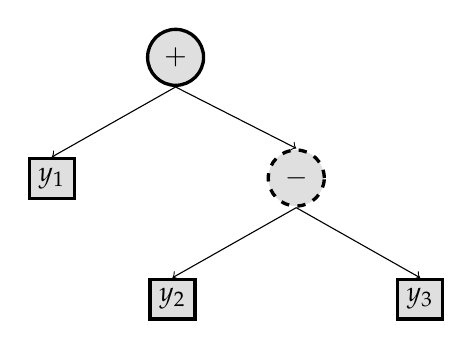
\begin{tikzpicture}[
                          roundnode_dashed/.style={circle, draw, dashed, fill=gray!25, very thick, minimum size=7mm},
                          roundnode/.style={circle, draw, fill=gray!25, very thick, minimum size=7mm},
                          squarednode/.style={rectangle, draw, fill=gray!25, very thick, minimum size=5mm},
                      ]
                      %Nodes
                      \node[roundnode]      (plus)                            {$+$};
                      \node[squarednode]    (y_1)     [below left=of plus]    {$y_1$};
                      \node[roundnode_dashed]      (sub)     [below right=of plus]   {$-$};
                      \node[squarednode]    (y_2)     [below left=of sub]     {$y_2$};
                      \node[squarednode]    (y_3)     [below right=of sub]    {$y_3$};


                      %   %Lines
                      \draw[->] (plus.south) -- (y_1.north);
                      \draw[->] (plus.south) -- (sub.north);
                      \draw[->] (sub.south) -- (y_2.north);
                      \draw[->] (sub.south) -- (y_3.north);
                  \end{tikzpicture}%
              \end{adjustbox}
              \qquad
              \begin{adjustbox}{width=0.25\textwidth, keepaspectratio}
                  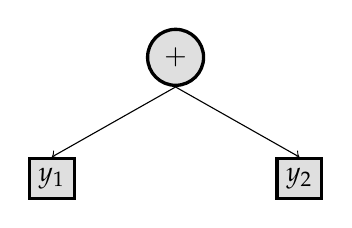
\begin{tikzpicture}[
                          roundnode_dashed/.style={circle, draw, dashed, fill=gray!25, very thick, minimum size=7mm},
                          roundnode/.style={circle, draw, fill=gray!25, very thick, minimum size=7mm},
                          squarednode/.style={rectangle, draw, fill=gray!25, very thick, minimum size=5mm},
                      ]
                      %Nodes
                      \node[roundnode]      (plus)                            {$+$};
                      \node[squarednode]    (y_1)     [below left=of plus]    {$y_1$};
                      \node[squarednode]    (y_2)     [below right=of plus]     {$y_2$};


                      %   %Lines
                      \draw[->] (plus.south) -- (y_1.north);
                      \draw[->] (plus.south) -- (y_2.north);
                  \end{tikzpicture}%
              \end{adjustbox}
          \end{center}

    \item Se cambia el nodo por uno nuevo que represente una operación aleatoria colocando como hijos nuevos árboles de expresiones aleatorias y como último hijo el nodo original que se seleccionó.

          Por ejempo, si se tiene el término $y_1 + (y_2 - y_3)$ se puede sustituir la resta por una multiplicación colocando como segundo factor la misma resta obteniéndose $y_1 + y_4 * (y_2 - y_3)$. Si se expresa en forma de árbol computacional sería:

          \begin{center}
              \begin{adjustbox}{width=0.25\textwidth, keepaspectratio}
                  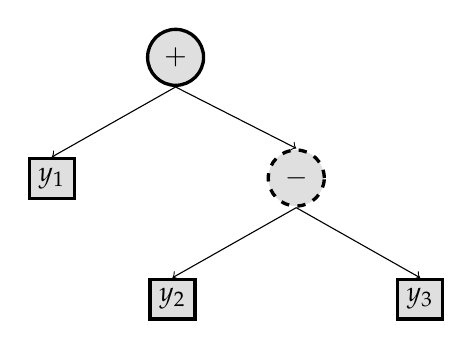
\begin{tikzpicture}[
                          roundnode_dashed/.style={circle, draw, dashed, fill=gray!25, very thick, minimum size=7mm},
                          roundnode/.style={circle, draw, fill=gray!25, very thick, minimum size=7mm},
                          squarednode/.style={rectangle, draw, fill=gray!25, very thick, minimum size=5mm},
                      ]
                      %Nodes
                      \node[roundnode]      (plus)                            {$+$};
                      \node[squarednode]    (y_1)     [below left=of plus]    {$y_1$};
                      \node[roundnode_dashed]      (sub)     [below right=of plus]   {$-$};
                      \node[squarednode]    (y_2)     [below left=of sub]     {$y_2$};
                      \node[squarednode]    (y_3)     [below right=of sub]    {$y_3$};


                      %   %Lines
                      \draw[->] (plus.south) -- (y_1.north);
                      \draw[->] (plus.south) -- (sub.north);
                      \draw[->] (sub.south) -- (y_2.north);
                      \draw[->] (sub.south) -- (y_3.north);
                  \end{tikzpicture}%
              \end{adjustbox}
              \qquad
              \begin{adjustbox}{width=0.25\textwidth, keepaspectratio}
                  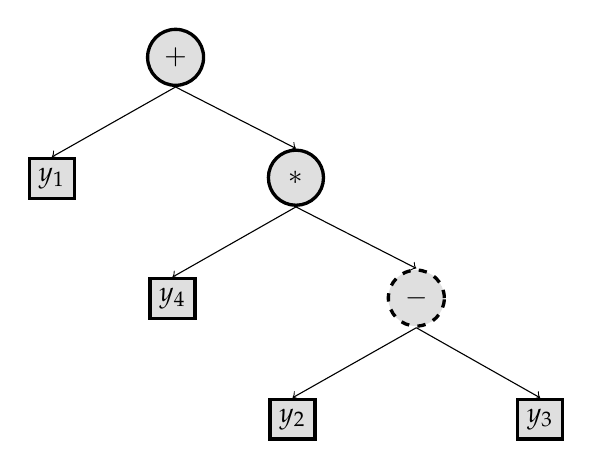
\begin{tikzpicture}[
                          roundnode_dashed/.style={circle, draw, dashed, fill=gray!25, very thick, minimum size=7mm},
                          roundnode/.style={circle, draw, fill=gray!25, very thick, minimum size=7mm},
                          squarednode/.style={rectangle, draw, fill=gray!25, very thick, minimum size=5mm},
                      ]
                      %Nodes
                      \node[roundnode]      (plus)                            {$+$};
                      \node[squarednode]    (y_1)     [below left=of plus]    {$y_1$};
                      \node[roundnode]    (star)  [below right=of plus]   {$*$};
                      \node[squarednode]  (y_4)   [below left=of star]        {$y_4$};
                      \node[roundnode_dashed]      (sub)     [below right=of star]   {$-$};
                      \node[squarednode]    (y_2)     [below left=of sub]     {$y_2$};
                      \node[squarednode]    (y_3)     [below right=of sub]    {$y_3$};


                      %   %Lines
                      \draw[->] (plus.south) -- (y_1.north);
                      \draw[->] (plus.south) -- (star.north);
                      \draw[->] (star.south) -- (y_4.north);
                      \draw[->] (star.south) -- (sub.north);
                      \draw[->] (sub.south) -- (y_2.north);
                      \draw[->] (sub.south) -- (y_3.north);
                  \end{tikzpicture}%
              \end{adjustbox}
          \end{center}

\end{itemize}

Si el nodo representa una variable:

\begin{itemize}
    \item Cambiar la variable por otra permitida dentro de la ecuación.

          Por ejempo, si se tiene el término $y_1 + (y_2 - y_3)$ se puede sustituir la variable $y_3$ resultando $y_1 + (y_2 - y_1)$. Si se plantea en forma de árbol computacional sería:

          \begin{center}
              \begin{adjustbox}{width=0.25\textwidth, keepaspectratio}
                  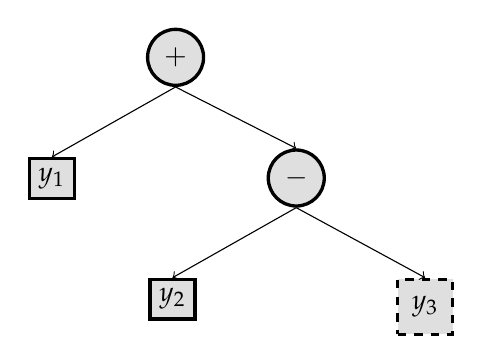
\begin{tikzpicture}[
                          roundnode/.style={circle, draw, fill=gray!25, very thick, minimum size=7mm},
                          squarednode/.style={rectangle, draw, fill=gray!25, very thick, minimum size=5mm},
                          squarednode_dashed/.style={rectangle, draw, dashed, fill=gray!25, very thick, minimum size=7mm},
                      ]
                      %Nodes
                      \node[roundnode]      (plus)                            {$+$};
                      \node[squarednode]    (y_1)     [below left=of plus]    {$y_1$};
                      \node[roundnode]      (sub)     [below right=of plus]   {$-$};
                      \node[squarednode]    (y_2)     [below left=of sub]     {$y_2$};
                      \node[squarednode_dashed]    (y_3)     [below right=of sub]    {$y_3$};


                      %   %Lines
                      \draw[->] (plus.south) -- (y_1.north);
                      \draw[->] (plus.south) -- (sub.north);
                      \draw[->] (sub.south) -- (y_2.north);
                      \draw[->] (sub.south) -- (y_3.north);
                  \end{tikzpicture}%
              \end{adjustbox}
              \qquad
              \begin{adjustbox}{width=0.25\textwidth, keepaspectratio}
                  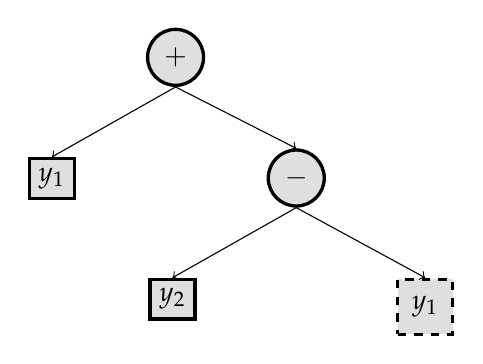
\begin{tikzpicture}[
                          roundnode/.style={circle, draw, fill=gray!25, very thick, minimum size=7mm},
                          squarednode/.style={rectangle, draw, fill=gray!25, very thick, minimum size=5mm},
                          squarednode_dashed/.style={rectangle, draw, dashed, fill=gray!25, very thick, minimum size=7mm},
                      ]
                      %Nodes
                      \node[roundnode]      (plus)                            {$+$};
                      \node[squarednode]    (y_1)     [below left=of plus]    {$y_1$};
                      \node[roundnode]      (sub)     [below right=of plus]   {$-$};
                      \node[squarednode]    (y_2)     [below left=of sub]     {$y_2$};
                      \node[squarednode_dashed]    (y_1_2)     [below right=of sub]    {$y_1$};


                      %   %Lines
                      \draw[->] (plus.south) -- (y_1.north);
                      \draw[->] (plus.south) -- (sub.north);
                      \draw[->] (sub.south) -- (y_2.north);
                      \draw[->] (sub.south) -- (y_1_2.north);
                  \end{tikzpicture}%
              \end{adjustbox}
          \end{center}

    \item Cambiar la variable por un nodo que represente una operación  aleatoria donde el primer hijo es la variable seleccionada.

          Por ejempo, si se tiene el término $y_1 + (y_2 - y_3)$ se puede sustituir la variable $y_3$ por una multiplicación donde el primer factor sea la misma variable $y_3$ resultando $y_1 + (y_2 - y_3 * y_2)$. Si se expresa en forma de árbol computacional sería:

          \begin{center}
              \begin{adjustbox}{width=0.25\textwidth, keepaspectratio}
                  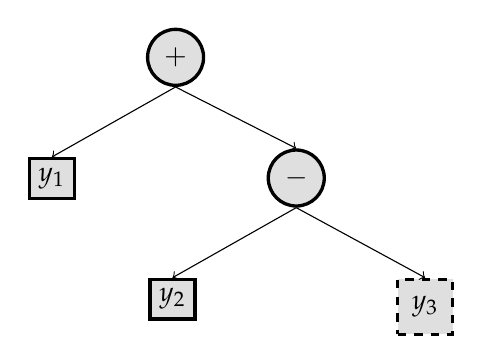
\begin{tikzpicture}[
                          roundnode/.style={circle, draw, fill=gray!25, very thick, minimum size=7mm},
                          squarednode/.style={rectangle, draw, fill=gray!25, very thick, minimum size=5mm},
                          squarednode_dashed/.style={rectangle, draw, dashed, fill=gray!25, very thick, minimum size=7mm},
                      ]
                      %Nodes
                      \node[roundnode]      (plus)                            {$+$};
                      \node[squarednode]    (y_1)     [below left=of plus]    {$y_1$};
                      \node[roundnode]      (sub)     [below right=of plus]   {$-$};
                      \node[squarednode]    (y_2)     [below left=of sub]     {$y_2$};
                      \node[squarednode_dashed]    (y_3)     [below right=of sub]    {$y_3$};


                      %   %Lines
                      \draw[->] (plus.south) -- (y_1.north);
                      \draw[->] (plus.south) -- (sub.north);
                      \draw[->] (sub.south) -- (y_2.north);
                      \draw[->] (sub.south) -- (y_3.north);
                  \end{tikzpicture}%
              \end{adjustbox}
              \qquad
              \begin{adjustbox}{width=0.25\textwidth, keepaspectratio}
                  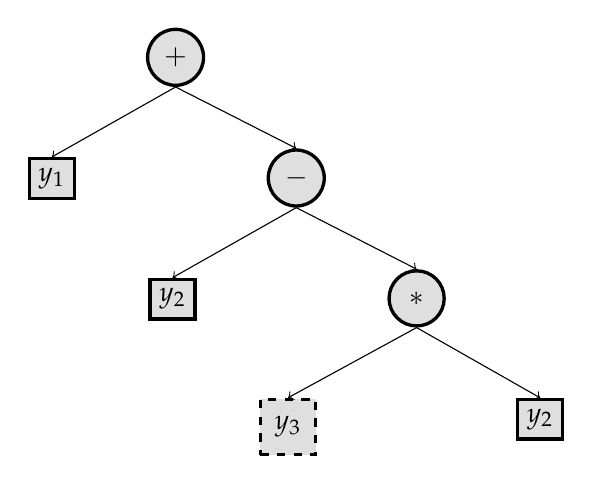
\begin{tikzpicture}[
                          roundnode/.style={circle, draw, fill=gray!25, very thick, minimum size=7mm},
                          squarednode/.style={rectangle, draw, fill=gray!25, very thick, minimum size=5mm},
                          squarednode_dashed/.style={rectangle, draw, dashed, fill=gray!25, very thick, minimum size=7mm},
                      ]
                      %Nodes
                      \node[roundnode]      (plus)                            {$+$};
                      \node[squarednode]    (y_1)     [below left=of plus]    {$y_1$};
                      \node[roundnode]    (sub)  [below right=of plus]   {$-$};
                      \node[squarednode]  (y_2)   [below left=of sub]        {$y_2$};
                      \node[roundnode]      (star)     [below right=of sub]   {$*$};
                      \node[squarednode_dashed]    (y_3)     [below left=of star]    {$y_3$};
                      \node[squarednode]    (y_2_2)     [below right=of star]     {$y_2$};


                      %   %Lines
                      \draw[->] (plus.south) -- (y_1.north);
                      \draw[->] (plus.south) -- (sub.north);
                      \draw[->] (sub.south) -- (y_2.north);
                      \draw[->] (sub.south) -- (star.north);
                      \draw[->] (star.south) -- (y_3.north);
                      \draw[->] (star.south) -- (y_2_2.north);
                  \end{tikzpicture}%
              \end{adjustbox}
          \end{center}

\end{itemize}

Como ejemplo de una operación de mutación se puede tomar el sistema:

\begin{align*}
    S' & = - a_1 * S * I         \\
    I' & = a_2 * S * I - a_3 * I \\
    R' & = a_4 * I,
\end{align*}

que se representa en forma de árbol computacional como:

\begin{center}
    \begin{adjustbox}{width=0.5\textwidth, keepaspectratio}
        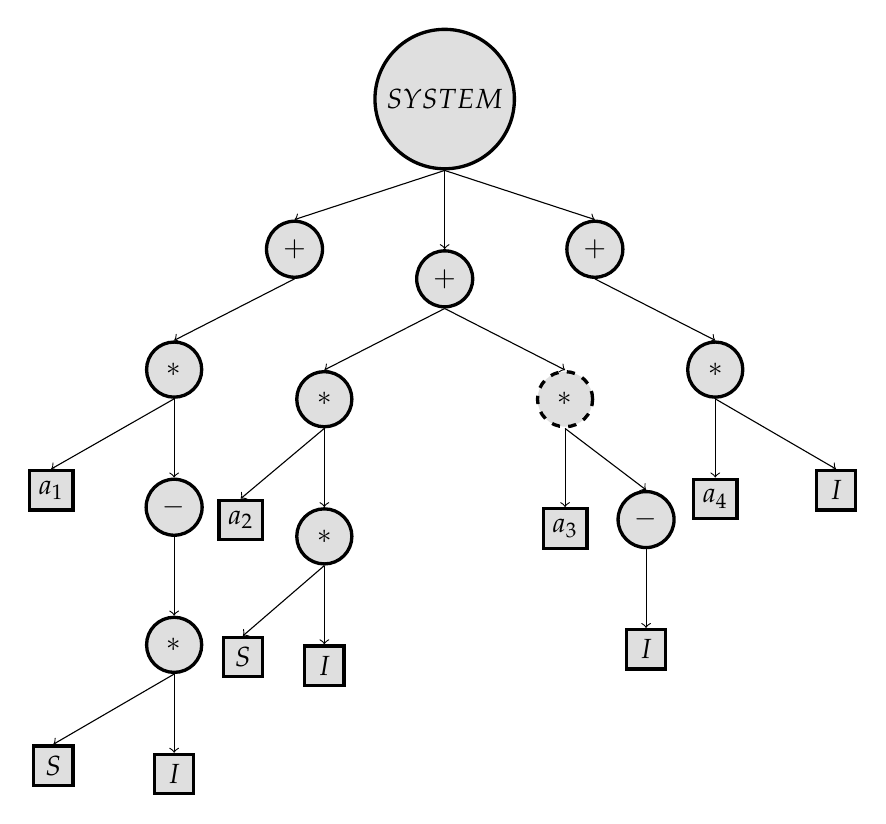
\begin{tikzpicture}[
                roundnode/.style={circle, draw, fill=gray!25, very thick, minimum size=7mm},
                squarednode/.style={rectangle, draw, fill=gray!25, very thick, minimum size=5mm},
                roundnode_dashed/.style={circle, draw, dashed, fill=gray!25, very thick, minimum size=7mm},
            ]
            % Nodes
            \node[roundnode]        (system)                            {$SYSTEM$};

            \node[roundnode]        (plus_S)     [below left=of system]        {$+$};
            \node[roundnode]        (star_S_1)    [below left=of plus_S]    {$*$};
            \node[squarednode]      (alpha_star_S_1)      [below left=of star_S_1]    {$a_1$};
            \node[roundnode]        (neg_star_S_1)    [below=of star_S_1]    {$-$};
            \node[roundnode]        (star_S_2)    [below=of neg_star_S_1]    {$*$};
            \node[squarednode]      (S_star_S)       [below left=of star_S_2]   {$S$};
            \node[squarednode]      (I_star_S)      [below=of star_S_2]   {$I$};

            \node[roundnode]        (plus_I)     [below=of system]        {$+$};
            \node[roundnode]        (star_I_1)    [below left=of plus_I]    {$*$};
            \node[squarednode]      (alpha_star_I_1)      [below left=1cm and 0.5cm of star_I_1]    {$a_2$};
            \node[roundnode]        (star_I_2)    [below=of star_I_1]    {$*$};
            \node[squarednode]      (S_star_I)       [below left=1cm and 0.5cm of star_I_2]   {$S$};
            \node[squarednode]      (I_star_I_1)      [below=of star_I_2]   {$I$};

            \node[roundnode_dashed]        (star_I_3)    [below right=of plus_I]    {$*$};
            \node[squarednode]      (beta_star_I_1)      [below=of star_I_3]    {$a_3$};
            \node[roundnode]        (neg_star_I_1)    [below right=1cm and 0.5cm of star_I_3]    {$-$};
            \node[squarednode]      (I_star_I_2)      [below=of neg_star_I_1]   {$I$};

            \node[roundnode]        (plus_R)     [below right=of system]        {$+$};
            \node[roundnode]        (star_R_1)    [below right=of plus_R]    {$*$};
            \node[squarednode]      (beta_star_R_1)      [below=of star_R_1]    {$a_4$};
            \node[squarednode]      (I_star_R)      [below right=of star_R_1]   {$I$};

            %Lines
            \draw [->] (system.south) -- (plus_S.north);
            \draw[->] (system.south) -- (plus_I.north);
            \draw[->] (system.south) -- (plus_R.north);

            \draw[->] (plus_S.south) -- (star_S_1.north);
            \draw[->] (star_S_1.south) -- (alpha_star_S_1.north);
            \draw[->] (star_S_1.south) -- (neg_star_S_1.north);
            \draw[->] (neg_star_S_1.south) -- (star_S_2.north);
            \draw[->] (star_S_2.south) -- (S_star_S.north);
            \draw[->] (star_S_2.south) -- (I_star_S.north);

            \draw[->] (plus_I.south) -- (star_I_1.north);
            \draw[->] (plus_I.south) -- (star_I_3.north);
            \draw[->] (star_I_1.south) -- (alpha_star_I_1.north);
            \draw[->] (star_I_1.south) -- (star_I_2.north);
            \draw[->] (star_I_2.south) -- (S_star_I.north);
            \draw[->] (star_I_2.south) -- (I_star_I_1.north);

            \draw[->] (star_I_3.south) -- (beta_star_I_1.north);
            \draw[->] (star_I_3.south) -- (neg_star_I_1.north);
            \draw[->] (neg_star_I_1.south) -- (I_star_I_2.north);

            \draw[->] (plus_R.south) -- (star_R_1.north);
            \draw[->] (star_R_1.south) -- (beta_star_R_1.north);
            \draw[->] (star_R_1.south) -- (I_star_R.north);
        \end{tikzpicture}
    \end{adjustbox}
\end{center}

Se puede realizar la mutación de eliminar el segundo término de la segunda ecuación quedando como resultado el sistema

\begin{align*}
    S' & = - a_1 * S * I \\
    I' & = a_2 * S * I   \\
    R' & = a_4 * I,
\end{align*}

que si se plantea en forma de árbol computacional es:

\begin{center}
    \begin{adjustbox}{width=0.5\textwidth, keepaspectratio}
        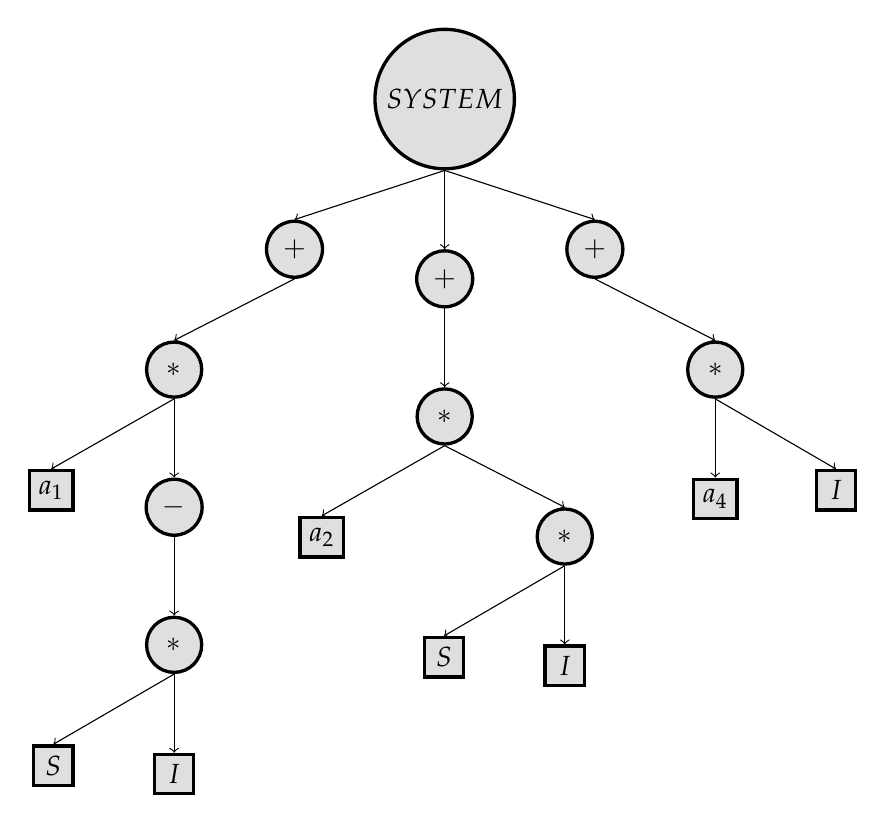
\begin{tikzpicture}[
                roundnode/.style={circle, draw, fill=gray!25, very thick, minimum size=7mm},
                squarednode/.style={rectangle, draw, fill=gray!25, very thick, minimum size=5mm},
                roundnode_dashed/.style={circle, draw, dashed, fill=gray!25, very thick, minimum size=7mm},
            ]
            % Nodes
            \node[roundnode]        (system)                            {$SYSTEM$};

            \node[roundnode]        (plus_S)     [below left=of system]        {$+$};
            \node[roundnode]        (star_S_1)    [below left=of plus_S]    {$*$};
            \node[squarednode]      (alpha_star_S_1)      [below left=of star_S_1]    {$a_1$};
            \node[roundnode]        (neg_star_S_1)    [below=of star_S_1]    {$-$};
            \node[roundnode]        (star_S_2)    [below=of neg_star_S_1]    {$*$};
            \node[squarednode]      (S_star_S)       [below left=of star_S_2]   {$S$};
            \node[squarednode]      (I_star_S)      [below=of star_S_2]   {$I$};

            \node[roundnode]        (plus_I)     [below=of system]        {$+$};
            \node[roundnode]        (star_I_1)    [below=of plus_I]    {$*$};
            \node[squarednode]      (alpha_star_I_1)      [below left=of star_I_1]    {$a_2$};
            \node[roundnode]        (star_I_2)    [below right=of star_I_1]    {$*$};
            \node[squarednode]      (S_star_I)       [below left=of star_I_2]   {$S$};
            \node[squarednode]      (I_star_I_1)      [below=of star_I_2]   {$I$};

            \node[roundnode]        (plus_R)     [below right=of system]        {$+$};
            \node[roundnode]        (star_R_1)    [below right=of plus_R]    {$*$};
            \node[squarednode]      (beta_star_R_1)      [below=of star_R_1]    {$a_4$};
            \node[squarednode]      (I_star_R)      [below right=of star_R_1]   {$I$};

            %Lines
            \draw [->] (system.south) -- (plus_S.north);
            \draw[->] (system.south) -- (plus_I.north);
            \draw[->] (system.south) -- (plus_R.north);

            \draw[->] (plus_S.south) -- (star_S_1.north);
            \draw[->] (star_S_1.south) -- (alpha_star_S_1.north);
            \draw[->] (star_S_1.south) -- (neg_star_S_1.north);
            \draw[->] (neg_star_S_1.south) -- (star_S_2.north);
            \draw[->] (star_S_2.south) -- (S_star_S.north);
            \draw[->] (star_S_2.south) -- (I_star_S.north);

            \draw[->] (plus_I.south) -- (star_I_1.north);
            \draw[->] (star_I_1.south) -- (alpha_star_I_1.north);
            \draw[->] (star_I_1.south) -- (star_I_2.north);
            \draw[->] (star_I_2.south) -- (S_star_I.north);
            \draw[->] (star_I_2.south) -- (I_star_I_1.north);

            \draw[->] (plus_R.south) -- (star_R_1.north);
            \draw[->] (star_R_1.south) -- (beta_star_R_1.north);
            \draw[->] (star_R_1.south) -- (I_star_R.north);
        \end{tikzpicture}
    \end{adjustbox}
\end{center}

Con estas modificaciones que pueden ocurrir en un sistema de ecuaciones diferenciales lineales en los parámetros se define la operación de mutación que se utiliza en el algoritmo genético que se emplea en este trabajo. Otra de las operaciones que se deben definir con el fin de implementar un algoritmo genético es el cruzamiento, que se describe en la siguiente sección.

\section{Cruzamiento}\label{section:xcross}

En la operación de cruzamiento se obtiene un nuevo sistema de ecuaciones diferenciales combinando propiedades de dos sistemas existentes A y B. Esta operación selecciona un nodo aleatorio dentro del árbol A y un nodo dentro del árbol B siguiendo un conjunto de reglas. Una vez escogidos los nodos se remplaza el subárbol del nodo seleccionado en A por el subárbol del nodo seleccionado en B, resultando en A un nuevo sistema de ecuaciones diferenciales.

Se impide que la selección tome hojas que representen parámetros. En dependencia de la altura del nodo seleccionado en A se escoge el nodo en B siguiendo las siguientes reglas:


\begin{itemize}
    \item Si el nodo seleccionado en A es el representante de la i-ésima ecuación en el sistema, se escoge el nodo representante de la i-ésima ecuación en el sistema B:

          \begin{center}
              \begin{adjustbox}{width=0.4\textwidth, keepaspectratio}
                  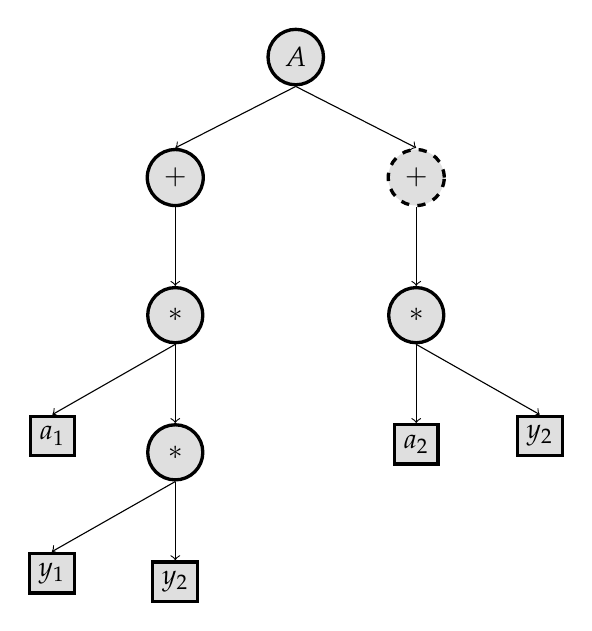
\begin{tikzpicture}[
                          roundnode/.style={circle, draw, fill=gray!25, very thick, minimum size=7mm},
                          squarednode/.style={rectangle, draw, fill=gray!25, very thick, minimum size=5mm},
                          roundnode_dashed/.style={circle, draw, dashed, fill=gray!25, very thick, minimum size=7mm},
                      ]
                      % Nodes
                      \node[roundnode]        (system)                            {$A$};

                      \node[roundnode]        (plus_1)     [below left=of system]        {$+$};
                      \node[roundnode]        (star_1_1)    [below=of plus_1]    {$*$};
                      \node[squarednode]      (a_1)      [below left=of star_1_1]    {$a_1$};
                      \node[roundnode]        (star_1_2)    [below=of star_1_1]    {$*$};
                      \node[squarednode]      (S_star_1_2)       [below left=of star_1_2]   {$y_1$};
                      \node[squarednode]      (I_star_1_2)      [below=of star_1_2]   {$y_2$};

                      \node[roundnode_dashed]        (plus_2)     [below right=of system]        {$+$};
                      \node[roundnode]        (star_2_1)    [below=of plus_2]    {$*$};
                      \node[squarednode]      (a_2)      [below=of star_2_1]    {$a_2$};
                      \node[squarednode]      (I_star_2_1)      [below right=of star_2_1]   {$y_2$};

                      %Lines
                      \draw [->] (system.south) -- (plus_1.north);
                      \draw[->] (system.south) -- (plus_2.north);
                      \draw[->] (plus_1.south) -- (star_1_1.north);
                      \draw[->] (plus_2.south) -- (star_2_1.north);
                      \draw[->] (star_1_1.south) -- (a_1.north);
                      \draw[->] (star_1_1.south) -- (star_1_2.north);
                      \draw[->] (star_1_2.south) -- (S_star_1_2.north);
                      \draw[->] (star_1_2.south) -- (I_star_1_2.north);
                      \draw[->] (star_2_1.south) -- (a_2.north);
                      \draw[->] (star_2_1.south) -- (I_star_2_1.north);
                  \end{tikzpicture}
              \end{adjustbox}
              \qquad
              \begin{adjustbox}{width=0.4\textwidth, keepaspectratio}
                  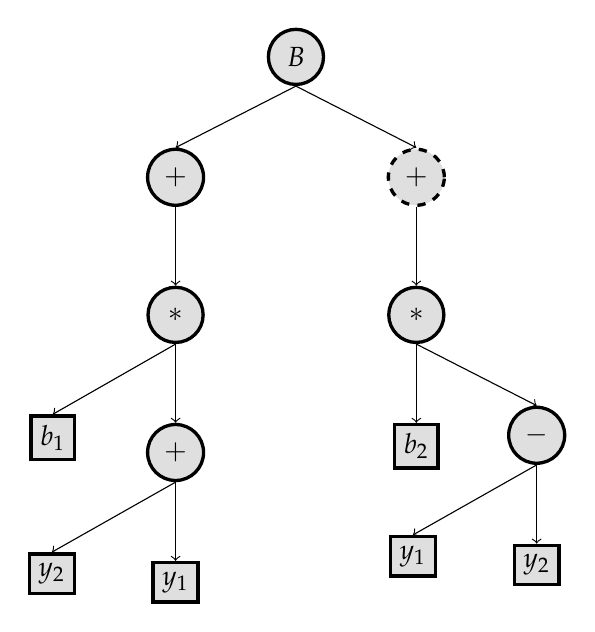
\begin{tikzpicture}[
                          roundnode/.style={circle, draw, fill=gray!25, very thick, minimum size=7mm},
                          squarednode/.style={rectangle, draw, fill=gray!25, very thick, minimum size=5mm},
                          roundnode_dashed/.style={circle, draw, dashed, fill=gray!25, very thick, minimum size=7mm},
                      ]
                      % Nodes
                      \node[roundnode]        (system)                            {$B$};

                      \node[roundnode]        (plus_1)     [below left=of system]        {$+$};
                      \node[roundnode]        (star_1_1)    [below=of plus_1]    {$*$};
                      \node[squarednode]      (a_3)      [below left=of star_1_1]    {$b_1$};
                      \node[roundnode]        (plus_1_2)    [below=of star_1_1]    {$+$};
                      \node[squarednode]      (I_plus_1_2)       [below left=of plus_1_2]   {$y_2$};
                      \node[squarednode]      (S_plus_1_2)      [below=of plus_1_2]   {$y_1$};

                      \node[roundnode_dashed]        (plus_2)     [below right=of system]        {$+$};
                      \node[roundnode]        (star_2_1)    [below=of plus_2]    {$*$};
                      \node[squarednode]      (a_4)      [below=of star_2_1]    {$b_2$};
                      \node[roundnode]        (sub_2_1)    [below right=of star_2_1]    {$-$};
                      \node[squarednode]      (S_sub_2_1)       [below left=of sub_2_1]   {$y_1$};
                      \node[squarednode]      (I_sub_2_1)      [below=of sub_2_1]   {$y_2$};

                      %Lines
                      \draw [->] (system.south) -- (plus_1.north);
                      \draw[->] (system.south) -- (plus_2.north);
                      \draw[->] (plus_1.south) -- (star_1_1.north);
                      \draw[->] (plus_2.south) -- (star_2_1.north);
                      \draw[->] (star_1_1.south) -- (a_3.north);
                      \draw[->] (star_1_1.south) -- (plus_1_2.north);
                      \draw[->] (plus_1_2.south) -- (I_plus_1_2.north);
                      \draw[->] (plus_1_2.south) -- (S_plus_1_2.north);
                      \draw[->] (star_2_1.south) -- (a_4.north);
                      \draw[->] (star_2_1.south) -- (sub_2_1.north);
                      \draw[->] (sub_2_1.south) -- (S_sub_2_1.north);
                      \draw[->] (sub_2_1.south) -- (I_sub_2_1.north);
                  \end{tikzpicture}
              \end{adjustbox}
          \end{center}

    \item Si se selecciona en A un nodo representante de un término en la ecuación i-ésima, se escoge un nodo representante de un término en la i-ésima ecuación en el sistema B:

          \begin{center}
              \begin{adjustbox}{width=0.4\textwidth, keepaspectratio}
                  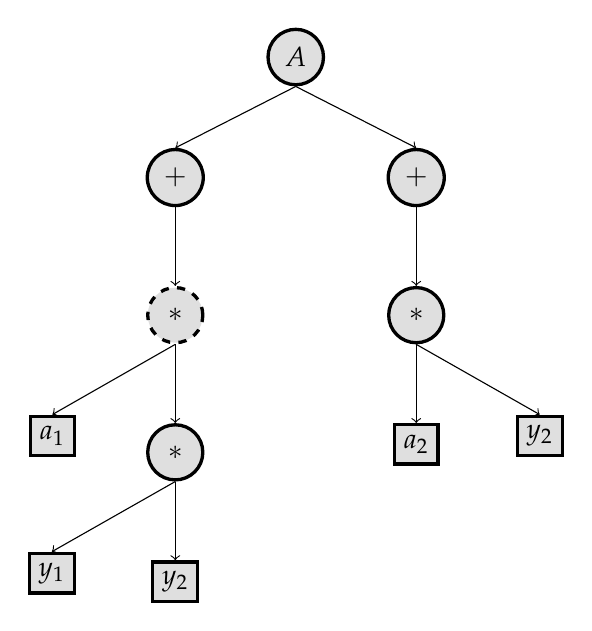
\begin{tikzpicture}[
                          roundnode/.style={circle, draw, fill=gray!25, very thick, minimum size=7mm},
                          squarednode/.style={rectangle, draw, fill=gray!25, very thick, minimum size=5mm},
                          roundnode_dashed/.style={circle, draw, dashed, fill=gray!25, very thick, minimum size=7mm},
                      ]
                      % Nodes
                      \node[roundnode]        (system)                            {$A$};

                      \node[roundnode]        (plus_1)     [below left=of system]        {$+$};
                      \node[roundnode_dashed]        (star_1_1)    [below=of plus_1]    {$*$};
                      \node[squarednode]      (a_1)      [below left=of star_1_1]    {$a_1$};
                      \node[roundnode]        (star_1_2)    [below=of star_1_1]    {$*$};
                      \node[squarednode]      (S_star_1_2)       [below left=of star_1_2]   {$y_1$};
                      \node[squarednode]      (I_star_1_2)      [below=of star_1_2]   {$y_2$};

                      \node[roundnode]        (plus_2)     [below right=of system]        {$+$};
                      \node[roundnode]        (star_2_1)    [below=of plus_2]    {$*$};
                      \node[squarednode]      (a_2)      [below=of star_2_1]    {$a_2$};
                      \node[squarednode]      (I_star_2_1)      [below right=of star_2_1]   {$y_2$};

                      %Lines
                      \draw [->] (system.south) -- (plus_1.north);
                      \draw[->] (system.south) -- (plus_2.north);
                      \draw[->] (plus_1.south) -- (star_1_1.north);
                      \draw[->] (plus_2.south) -- (star_2_1.north);
                      \draw[->] (star_1_1.south) -- (a_1.north);
                      \draw[->] (star_1_1.south) -- (star_1_2.north);
                      \draw[->] (star_1_2.south) -- (S_star_1_2.north);
                      \draw[->] (star_1_2.south) -- (I_star_1_2.north);
                      \draw[->] (star_2_1.south) -- (a_2.north);
                      \draw[->] (star_2_1.south) -- (I_star_2_1.north);
                  \end{tikzpicture}
              \end{adjustbox}
              \qquad
              \begin{adjustbox}{width=0.4\textwidth, keepaspectratio}
                  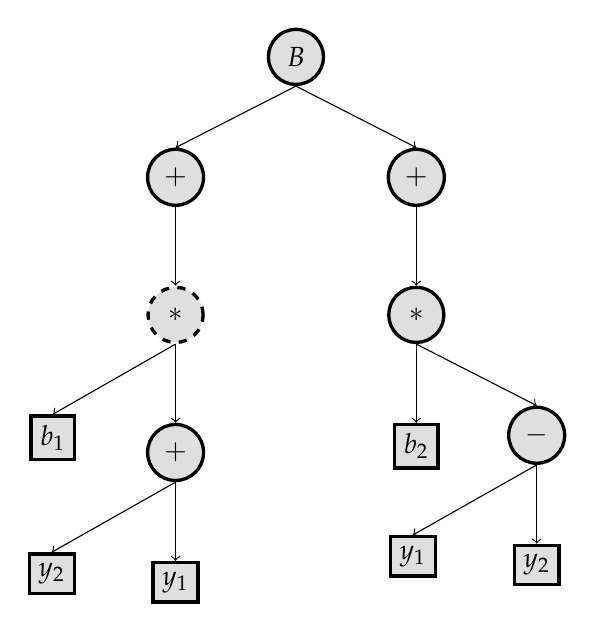
\begin{tikzpicture}[
                          roundnode/.style={circle, draw, fill=gray!25, very thick, minimum size=7mm},
                          squarednode/.style={rectangle, draw, fill=gray!25, very thick, minimum size=5mm},
                          roundnode_dashed/.style={circle, draw, dashed, fill=gray!25, very thick, minimum size=7mm},
                      ]
                      % Nodes
                      \node[roundnode]        (system)                            {$B$};

                      \node[roundnode]        (plus_1)     [below left=of system]        {$+$};
                      \node[roundnode_dashed]        (star_1_1)    [below=of plus_1]    {$*$};
                      \node[squarednode]      (a_3)      [below left=of star_1_1]    {$b_1$};
                      \node[roundnode]        (plus_1_2)    [below=of star_1_1]    {$+$};
                      \node[squarednode]      (I_plus_1_2)       [below left=of plus_1_2]   {$y_2$};
                      \node[squarednode]      (S_plus_1_2)      [below=of plus_1_2]   {$y_1$};

                      \node[roundnode]        (plus_2)     [below right=of system]        {$+$};
                      \node[roundnode]        (star_2_1)    [below=of plus_2]    {$*$};
                      \node[squarednode]      (a_4)      [below=of star_2_1]    {$b_2$};
                      \node[roundnode]        (sub_2_1)    [below right=of star_2_1]    {$-$};
                      \node[squarednode]      (S_sub_2_1)       [below left=of sub_2_1]   {$y_1$};
                      \node[squarednode]      (I_sub_2_1)      [below=of sub_2_1]   {$y_2$};

                      %Lines
                      \draw [->] (system.south) -- (plus_1.north);
                      \draw[->] (system.south) -- (plus_2.north);
                      \draw[->] (plus_1.south) -- (star_1_1.north);
                      \draw[->] (plus_2.south) -- (star_2_1.north);
                      \draw[->] (star_1_1.south) -- (a_3.north);
                      \draw[->] (star_1_1.south) -- (plus_1_2.north);
                      \draw[->] (plus_1_2.south) -- (I_plus_1_2.north);
                      \draw[->] (plus_1_2.south) -- (S_plus_1_2.north);
                      \draw[->] (star_2_1.south) -- (a_4.north);
                      \draw[->] (star_2_1.south) -- (sub_2_1.north);
                      \draw[->] (sub_2_1.south) -- (S_sub_2_1.north);
                      \draw[->] (sub_2_1.south) -- (I_sub_2_1.north);
                  \end{tikzpicture}
              \end{adjustbox}
          \end{center}


    \item Si el nodo seleccionado en A es el representante de una operación o una variable perteneciente a la i-ésima ecuación, se selecciona un nodo representante de una operación o una variable que pertenezca a algún término en la i-ésima ecuación en el sistema B:


          \begin{center}
              \begin{adjustbox}{width=0.4\textwidth, keepaspectratio}
                  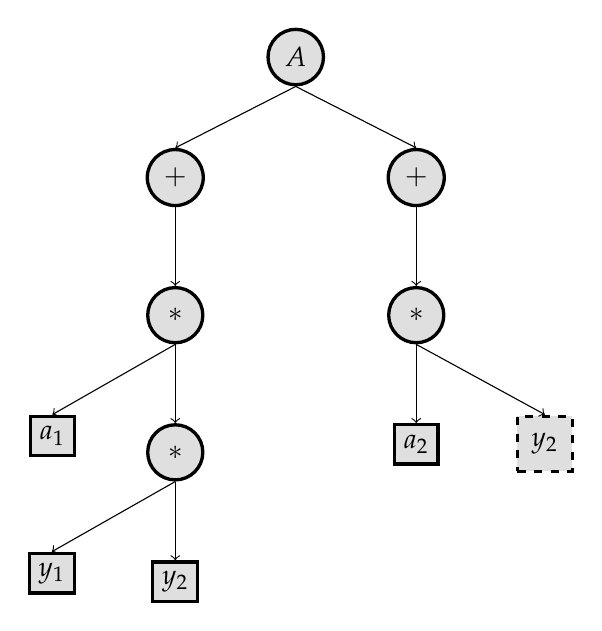
\begin{tikzpicture}[
                          roundnode/.style={circle, draw, fill=gray!25, very thick, minimum size=7mm},
                          squarednode/.style={rectangle, draw, fill=gray!25, very thick, minimum size=5mm},
                          squarednode_dashed/.style={rectangle, draw, dashed, fill=gray!25, very thick, minimum size=7mm},
                      ]
                      % Nodes
                      \node[roundnode]        (system)                            {$A$};

                      \node[roundnode]        (plus_1)     [below left=of system]        {$+$};
                      \node[roundnode]        (star_1_1)    [below=of plus_1]    {$*$};
                      \node[squarednode]      (a_1)      [below left=of star_1_1]    {$a_1$};
                      \node[roundnode]        (star_1_2)    [below=of star_1_1]    {$*$};
                      \node[squarednode]      (S_star_1_2)       [below left=of star_1_2]   {$y_1$};
                      \node[squarednode]      (I_star_1_2)      [below=of star_1_2]   {$y_2$};

                      \node[roundnode]        (plus_2)     [below right=of system]        {$+$};
                      \node[roundnode]        (star_2_1)    [below=of plus_2]    {$*$};
                      \node[squarednode]      (a_2)      [below=of star_2_1]    {$a_2$};
                      \node[squarednode_dashed]      (I_star_2_1)      [below right=of star_2_1]   {$y_2$};

                      %Lines
                      \draw [->] (system.south) -- (plus_1.north);
                      \draw[->] (system.south) -- (plus_2.north);
                      \draw[->] (plus_1.south) -- (star_1_1.north);
                      \draw[->] (plus_2.south) -- (star_2_1.north);
                      \draw[->] (star_1_1.south) -- (a_1.north);
                      \draw[->] (star_1_1.south) -- (star_1_2.north);
                      \draw[->] (star_1_2.south) -- (S_star_1_2.north);
                      \draw[->] (star_1_2.south) -- (I_star_1_2.north);
                      \draw[->] (star_2_1.south) -- (a_2.north);
                      \draw[->] (star_2_1.south) -- (I_star_2_1.north);
                  \end{tikzpicture}
              \end{adjustbox}
              \qquad
              \begin{adjustbox}{width=0.4\textwidth, keepaspectratio}
                  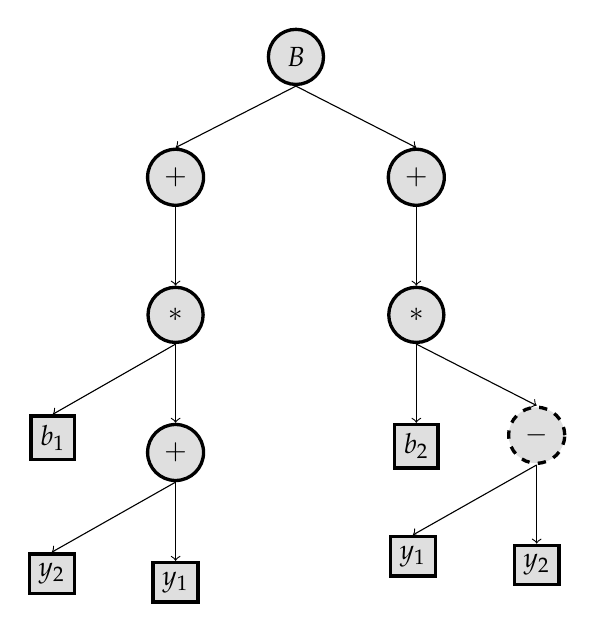
\begin{tikzpicture}[
                          roundnode/.style={circle, draw, fill=gray!25, very thick, minimum size=7mm},
                          squarednode/.style={rectangle, draw, fill=gray!25, very thick, minimum size=5mm},
                          roundnode_dashed/.style={circle, draw, dashed, fill=gray!25, very thick, minimum size=7mm},
                      ]
                      % Nodes
                      \node[roundnode]        (system)                            {$B$};

                      \node[roundnode]        (plus_1)     [below left=of system]        {$+$};
                      \node[roundnode]        (star_1_1)    [below=of plus_1]    {$*$};
                      \node[squarednode]      (a_3)      [below left=of star_1_1]    {$b_1$};
                      \node[roundnode]        (plus_1_2)    [below=of star_1_1]    {$+$};
                      \node[squarednode]      (I_plus_1_2)       [below left=of plus_1_2]   {$y_2$};
                      \node[squarednode]      (S_plus_1_2)      [below=of plus_1_2]   {$y_1$};

                      \node[roundnode]        (plus_2)     [below right=of system]        {$+$};
                      \node[roundnode]        (star_2_1)    [below=of plus_2]    {$*$};
                      \node[squarednode]      (a_4)      [below=of star_2_1]    {$b_2$};
                      \node[roundnode_dashed]        (sub_2_1)    [below right=of star_2_1]    {$-$};
                      \node[squarednode]      (S_sub_2_1)       [below left=of sub_2_1]   {$y_1$};
                      \node[squarednode]      (I_sub_2_1)      [below=of sub_2_1]   {$y_2$};

                      %Lines
                      \draw [->] (system.south) -- (plus_1.north);
                      \draw[->] (system.south) -- (plus_2.north);
                      \draw[->] (plus_1.south) -- (star_1_1.north);
                      \draw[->] (plus_2.south) -- (star_2_1.north);
                      \draw[->] (star_1_1.south) -- (a_3.north);
                      \draw[->] (star_1_1.south) -- (plus_1_2.north);
                      \draw[->] (plus_1_2.south) -- (I_plus_1_2.north);
                      \draw[->] (plus_1_2.south) -- (S_plus_1_2.north);
                      \draw[->] (star_2_1.south) -- (a_4.north);
                      \draw[->] (star_2_1.south) -- (sub_2_1.north);
                      \draw[->] (sub_2_1.south) -- (S_sub_2_1.north);
                      \draw[->] (sub_2_1.south) -- (I_sub_2_1.north);
                  \end{tikzpicture}
              \end{adjustbox}
          \end{center}

\end{itemize}

Por ejemplo, si se tiene el sistema

\begin{align*}
    S' & = - a_1 * S * I         \\
    I' & = a_2 * S * I - a_3 * I \\
    R' & = a_4 * I,
\end{align*}

que se representa con el árbol computacional:

\begin{center}
    \begin{adjustbox}{width=0.5\textwidth, keepaspectratio}
        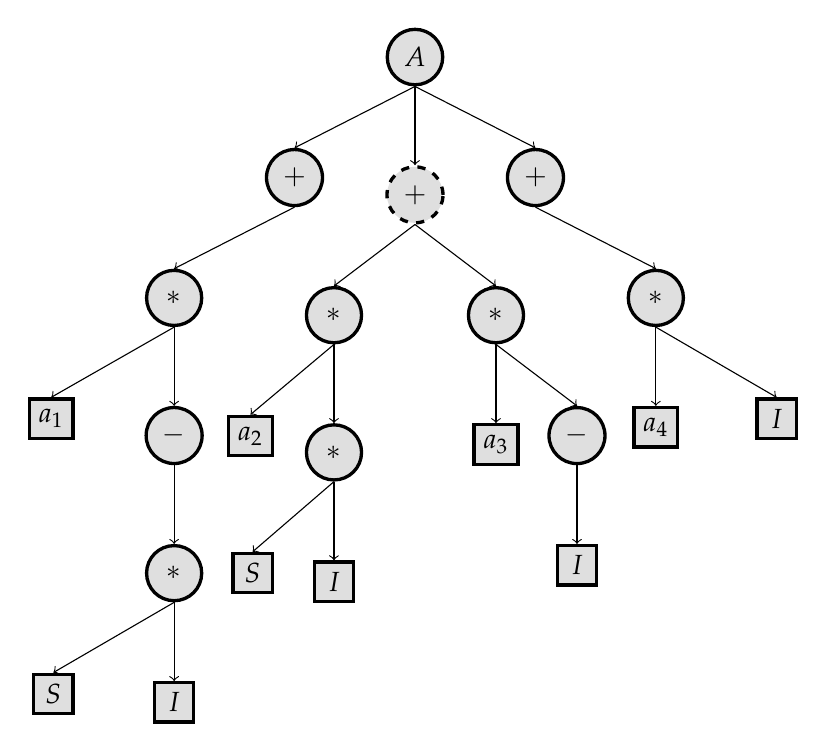
\begin{tikzpicture}[
                roundnode/.style={circle, draw, fill=gray!25, very thick, minimum size=7mm},
                squarednode/.style={rectangle, draw, fill=gray!25, very thick, minimum size=5mm},
                roundnode_dashed/.style={circle, draw, dashed, fill=gray!25, very thick, minimum size=7mm},
            ]
            % Nodes
            \node[roundnode]        (system)                            {$A$};

            \node[roundnode]        (plus_S)     [below left=of system]        {$+$};
            \node[roundnode]        (star_S_1)    [below left=of plus_S]    {$*$};
            \node[squarednode]      (alpha_star_S_1)      [below left=of star_S_1]    {$a_1$};
            \node[roundnode]        (neg_star_S_1)    [below=of star_S_1]    {$-$};
            \node[roundnode]        (star_S_2)    [below=of neg_star_S_1]    {$*$};
            \node[squarednode]      (S_star_S)       [below left=of star_S_2]   {$S$};
            \node[squarednode]      (I_star_S)      [below=of star_S_2]   {$I$};

            \node[roundnode_dashed]        (plus_I)     [below=of system]        {$+$};
            \node[roundnode]        (star_I_1)    [below left=1cm and 0.5cm of plus_I]    {$*$};
            \node[squarednode]      (alpha_star_I_1)      [below left=1cm and 0.5cm of star_I_1]    {$a_2$};
            \node[roundnode]        (star_I_2)    [below=of star_I_1]    {$*$};
            \node[squarednode]      (S_star_I)       [below left=1cm and 0.5cm of star_I_2]   {$S$};
            \node[squarednode]      (I_star_I_1)      [below=of star_I_2]   {$I$};

            \node[roundnode]        (star_I_3)    [below right=1cm and 0.5cm of plus_I]    {$*$};
            \node[squarednode]      (beta_star_I_1)      [below=of star_I_3]    {$a_3$};
            \node[roundnode]        (neg_star_I_1)    [below right=1cm and 0.5cm of star_I_3]    {$-$};
            \node[squarednode]      (I_star_I_2)      [below=of neg_star_I_1]   {$I$};

            \node[roundnode]        (plus_R)     [below right=of system]        {$+$};
            \node[roundnode]        (star_R_1)    [below right=of plus_R]    {$*$};
            \node[squarednode]      (beta_star_R_1)      [below=of star_R_1]    {$a_4$};
            \node[squarednode]      (I_star_R)      [below right=of star_R_1]   {$I$};

            %Lines
            \draw [->] (system.south) -- (plus_S.north);
            \draw[->] (system.south) -- (plus_I.north);
            \draw[->] (system.south) -- (plus_R.north);

            \draw[->] (plus_S.south) -- (star_S_1.north);
            \draw[->] (star_S_1.south) -- (alpha_star_S_1.north);
            \draw[->] (star_S_1.south) -- (neg_star_S_1.north);
            \draw[->] (neg_star_S_1.south) -- (star_S_2.north);
            \draw[->] (star_S_2.south) -- (S_star_S.north);
            \draw[->] (star_S_2.south) -- (I_star_S.north);

            \draw[->] (plus_I.south) -- (star_I_1.north);
            \draw[->] (plus_I.south) -- (star_I_3.north);
            \draw[->] (star_I_1.south) -- (alpha_star_I_1.north);
            \draw[->] (star_I_1.south) -- (star_I_2.north);
            \draw[->] (star_I_2.south) -- (S_star_I.north);
            \draw[->] (star_I_2.south) -- (I_star_I_1.north);

            \draw[->] (star_I_3.south) -- (beta_star_I_1.north);
            \draw[->] (star_I_3.south) -- (neg_star_I_1.north);
            \draw[->] (neg_star_I_1.south) -- (I_star_I_2.north);

            \draw[->] (plus_R.south) -- (star_R_1.north);
            \draw[->] (star_R_1.south) -- (beta_star_R_1.north);
            \draw[->] (star_R_1.south) -- (I_star_R.north);
        \end{tikzpicture}
    \end{adjustbox}
\end{center}

y el sistema

\begin{align*}
    S' & = b_1 * (S + I) \\
    I' & = b_2 * S * I   \\
    R' & = b_3 * S,
\end{align*}

que su representación en forma de árbol computacional es:

\begin{center}
    \begin{adjustbox}{width=0.5\textwidth, keepaspectratio}
        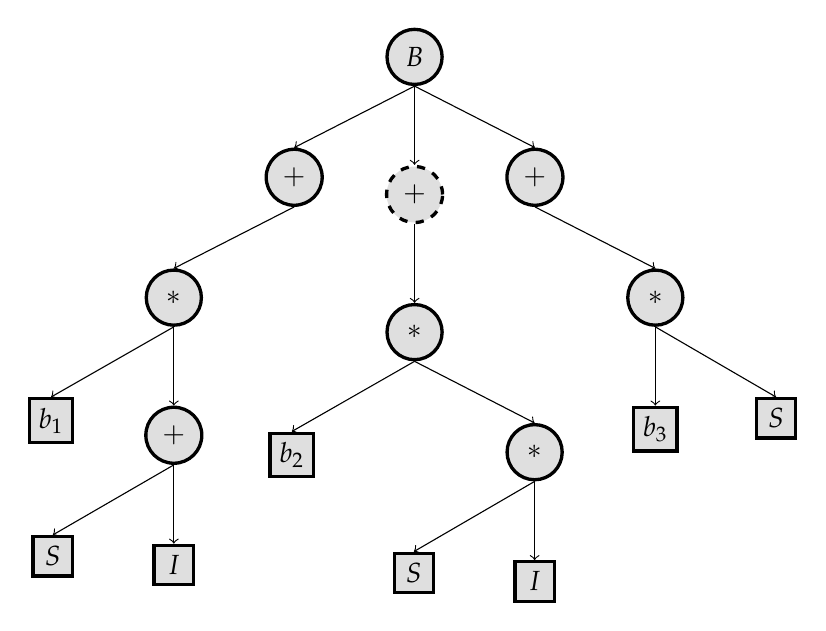
\begin{tikzpicture}[
                roundnode/.style={circle, draw, fill=gray!25, very thick, minimum size=7mm},
                squarednode/.style={rectangle, draw, fill=gray!25, very thick, minimum size=5mm},
                roundnode_dashed/.style={circle, draw, dashed, fill=gray!25, very thick, minimum size=7mm},
            ]
            % Nodes
            \node[roundnode]        (system)                            {$B$};

            \node[roundnode]        (plus_S)     [below left=of system]        {$+$};
            \node[roundnode]        (star_S_1)    [below left=of plus_S]    {$*$};
            \node[squarednode]      (alpha_star_S_1)      [below left=of star_S_1]    {$b_1$};
            \node[roundnode]        (add_S_2)    [below=of star_S_1]    {$+$};
            \node[squarednode]      (S_star_S)       [below left=of add_S_2]   {$S$};
            \node[squarednode]      (I_star_S)      [below=of add_S_2]   {$I$};

            \node[roundnode_dashed]        (plus_I)     [below=of system]        {$+$};
            \node[roundnode]        (star_I_1)    [below=of plus_I]    {$*$};
            \node[squarednode]      (alpha_star_I_1)      [below left=of star_I_1]    {$b_2$};
            \node[roundnode]        (star_I_2)    [below right=of star_I_1]    {$*$};
            \node[squarednode]      (S_star_I)       [below left=of star_I_2]   {$S$};
            \node[squarednode]      (I_star_I_1)      [below=of star_I_2]   {$I$};

            \node[roundnode]        (plus_R)     [below right=of system]        {$+$};
            \node[roundnode]        (star_R_1)    [below right=of plus_R]    {$*$};
            \node[squarednode]      (beta_star_R_1)      [below=of star_R_1]    {$b_3$};
            \node[squarednode]      (S_star_R)      [below right=of star_R_1]   {$S$};

            %Lines
            \draw [->] (system.south) -- (plus_S.north);
            \draw[->] (system.south) -- (plus_I.north);
            \draw[->] (system.south) -- (plus_R.north);

            \draw[->] (plus_S.south) -- (star_S_1.north);
            \draw[->] (star_S_1.south) -- (alpha_star_S_1.north);
            \draw[->] (star_S_1.south) -- (add_S_2.north);
            \draw[->] (add_S_2.south) -- (S_star_S.north);
            \draw[->] (add_S_2.south) -- (I_star_S.north);

            \draw[->] (plus_I.south) -- (star_I_1.north);
            \draw[->] (star_I_1.south) -- (alpha_star_I_1.north);
            \draw[->] (star_I_1.south) -- (star_I_2.north);
            \draw[->] (star_I_2.south) -- (S_star_I.north);
            \draw[->] (star_I_2.south) -- (I_star_I_1.north);

            \draw[->] (plus_R.south) -- (star_R_1.north);
            \draw[->] (star_R_1.south) -- (beta_star_R_1.north);
            \draw[->] (star_R_1.south) -- (S_star_R.north);
        \end{tikzpicture}
    \end{adjustbox}
\end{center}

y como resultado de la operación de cruzamiento los nodos seleccionados son los que se resaltan con líneas discontinuas, entonces el sistema resultante sería

\begin{align*}
    S' & = - a_1 * S * I \\
    I' & = b_2 * S * I   \\
    R' & = a_4 * I,
\end{align*}

que se representa con el árbol computacional:

\begin{center}
    \begin{adjustbox}{width=0.5\textwidth, keepaspectratio}
        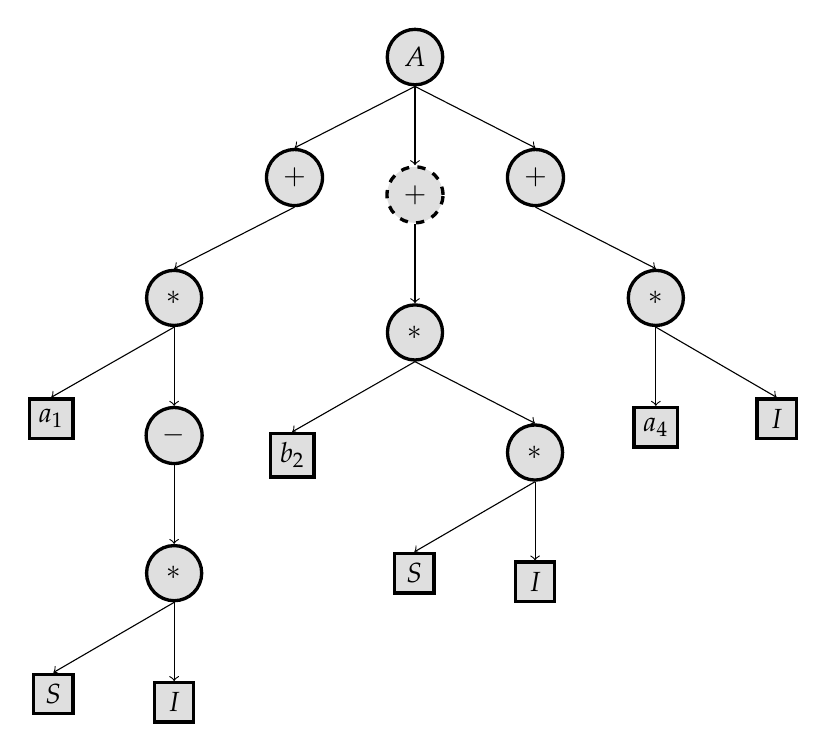
\begin{tikzpicture}[
                roundnode/.style={circle, draw, fill=gray!25, very thick, minimum size=7mm},
                squarednode/.style={rectangle, draw, fill=gray!25, very thick, minimum size=5mm},
                roundnode_dashed/.style={circle, draw, dashed, fill=gray!25, very thick, minimum size=7mm},
            ]
            % Nodes
            \node[roundnode]        (system)                            {$A$};

            \node[roundnode]        (plus_S)     [below left=of system]        {$+$};
            \node[roundnode]        (star_S_1)    [below left=of plus_S]    {$*$};
            \node[squarednode]      (alpha_star_S_1)      [below left=of star_S_1]    {$a_1$};
            \node[roundnode]        (neg_star_S_1)    [below=of star_S_1]    {$-$};
            \node[roundnode]        (star_S_2)    [below=of neg_star_S_1]    {$*$};
            \node[squarednode]      (S_star_S)       [below left=of star_S_2]   {$S$};
            \node[squarednode]      (I_star_S)      [below=of star_S_2]   {$I$};

            \node[roundnode_dashed]        (plus_I)     [below=of system]        {$+$};
            \node[roundnode]        (star_I_1)    [below=of plus_I]    {$*$};
            \node[squarednode]      (alpha_star_I_1)      [below left=of star_I_1]    {$b_2$};
            \node[roundnode]        (star_I_2)    [below right=of star_I_1]    {$*$};
            \node[squarednode]      (S_star_I)       [below left=of star_I_2]   {$S$};
            \node[squarednode]      (I_star_I_1)      [below=of star_I_2]   {$I$};

            \node[roundnode]        (plus_R)     [below right=of system]        {$+$};
            \node[roundnode]        (star_R_1)    [below right=of plus_R]    {$*$};
            \node[squarednode]      (beta_star_R_1)      [below=of star_R_1]    {$a_4$};
            \node[squarednode]      (I_star_R)      [below right=of star_R_1]   {$I$};

            %Lines
            \draw [->] (system.south) -- (plus_S.north);
            \draw[->] (system.south) -- (plus_I.north);
            \draw[->] (system.south) -- (plus_R.north);

            \draw[->] (plus_S.south) -- (star_S_1.north);
            \draw[->] (star_S_1.south) -- (alpha_star_S_1.north);
            \draw[->] (star_S_1.south) -- (neg_star_S_1.north);
            \draw[->] (neg_star_S_1.south) -- (star_S_2.north);
            \draw[->] (star_S_2.south) -- (S_star_S.north);
            \draw[->] (star_S_2.south) -- (I_star_S.north);

            \draw[->] (plus_I.south) -- (star_I_1.north);
            \draw[->] (star_I_1.south) -- (alpha_star_I_1.north);
            \draw[->] (star_I_1.south) -- (star_I_2.north);
            \draw[->] (star_I_2.south) -- (S_star_I.north);
            \draw[->] (star_I_2.south) -- (I_star_I_1.north);

            \draw[->] (plus_R.south) -- (star_R_1.north);
            \draw[->] (star_R_1.south) -- (beta_star_R_1.north);
            \draw[->] (star_R_1.south) -- (I_star_R.north);
        \end{tikzpicture}
    \end{adjustbox}
\end{center}

Una vez definidas las operaciones de mutación y cruzamiento solo faltaría detallar la operación de selección para tener totalmente definido el algoritmo genético. Los detalles de la última operación se presentan en la siguiente sección.

\section{Selección de las soluciones que pasan a la siguiente generación}\label{section:selection}

Dada una población inicial en una generación, se selecciona un subconjunto de individuos de la población y se mutan, y se toma otro subconjunto de individuos y se cruzan entre ellos. A partir de las operaciones de mutación y cruzamiento aparece un nuevo subconjunto de individuos. Este nuevo subconjunto se agrega a la población inicial de la generación, formando así un nuevo conjunto de individuos el cual se define como población total de la generación.

De la población total de la generación se seleccionan los individuos que mejor ajustan los datos. Se seleccionan también algunos individuos aleatorios con el fin de evitar mínimos locales en la búsqueda del mejor sistema. En total se selecciona de la población total de la generación una cantidad igual a la presente en la población inicial de la generación.

Como resultado de la selección se obtiene una nueva población que será la población de la siguiente generación. Las operaciones de mutación y cruzamiento de la población inicial y luego selección de individuos se repiten un número fijo de veces que se define mediante un parámetro del algoritmo. Esta repetición se realiza con el fin de generar varias generaciones intentando obtener mejores soluciones cada vez.

En este capítulo se describió cómo representar un sistema de EDOs lineal con respecto a los parámetros, cómo calcular su costo para un conjunto de datos, así como la forma de cruzar y mutar estos sistemas. Con estos elementos se puede definir un algoritmo genético para determinar el sistema de EDOs lineal con respecto a los parámetros que mejor describa un conjunto de datos.

En el siguiente capítulo se muestran los resultados obtenidos de aplicar la regresión simbólica que se plantea en varios conjuntos de puntos.
\include{MainMatter/Background}
\chapter{Experimentos y resultados}\label{chapter:results}

En este capítulo se presentan los experimentos realizados para evaluar el desempeño y los resultados de la regresión simbólica propuesta en este trabajo.

En la sección \ref{section:experimental_considerations} se describe el marco experimental. En \ref{section:experimental_frame} se muestra como se generaron los datos utilizados en los distintos experimentos y cómo se modeló la presencia de ruido en las muestras. En la sección \ref{section:experiments} se describen los experimentos realizados y sus resultados, y en \ref{section:experiments_results} se analizan. A continuación se describe el marco experimental.

\section{Consideraciones de la etapa de experimentación}\label{section:experimental_considerations}

El espacio de búsqueda en la regresión simbólica que se propone en este trabajo comprende a todos los sistemas de ecuaciones diferenciales lineales con respecto a los parámetros que se pueden formar con un conjunto predefinido de operaciones, y donde la cantidad de ecuaciones se define según los datos. La regresión simbólica es un problema NP-difícil por lo que resulta computacionalmente costoso. Para lidiar con este costo computacional se diseñó un marco experimental que fuese factible de ejecutar en un ordenador portátil. El equipo de cómputo donde se realizaron los experimentos posee las siguientes propiedades.

\begin{itemize}
    \item \textbf{Procesador}: 11th Gen intel i9-11900H @ 2.50GHz
    \item \textbf{RAM}: 40GB
    \item \textbf{Arquitectura}: 64 bits
\end{itemize}

La implementación de la solución se desarrolla en el lenguaje de programación \emph{Python} auxiliado por las bibliotecas \emph{numpy} \cite{harris2020array} y \emph{scipy} \cite{2020SciPy-NMeth} para la integración de los modelos y \emph{csaps} \cite{csaps} para eliminar ruido en los datos mediante un spline de suavizado. El algoritmo de regresión simbólica utilizado en los experimentos fue desarrollado durante la investigación y se encuentra en \textbf{GitHub} \cite{symbolic-regression}.

Como métrica para evaluar la calidad de la solución generada por la regresión simbólica se utiliza el error cuadrático medio. Menores valores de esta métrica implica que el valor de los datos evaluados en el sistema obtenido en la regresión simbólica se acercan a los datos observados.

Cada experimento que aparece en la sección \ref{section:experiments} se realizó 30 veces y se plantea el valor promedio que obtuvo la métrica utilizada en las 30 ejecuciones del experimento. Además se indica el valor mínimo y máximo que alcanzó la métrica a lo largo de los 30 experimentos. De igual forma se plantea cuántas veces en la realización de los 30 experimentos, el método de regresión simbólica encontró un sistema igual al usado para generar los datos.

En la siguiente sección se detalla cómo se generan los datos para realizar los distintos experimentos.

\section{Descripción del marco experimental}\label{section:experimental_frame}

Los experimentos inician con la selección de un modelo conocido $f$. Para ilustrar el proceso se asumirá que el sistema es el correspondiente al modelo SIR:

\begin{align*}
    S' & = - aIS    \\
    I' & = aIS - bI \\
    R' & = bI.
\end{align*}

El sistema de ecuaciones diferenciales se integra en un intervalo predefinido y se obtiene un conjunto de puntos que representan el valor de las distintas variables a lo largo del tiempo. Por ejemplo, si se integra el modelo SIR utilizando como parámetros $a = 0.3$, $b = 0.1$ y con $0 \leq t \leq 20$ se obtienen las curvas en la imagen \ref{fig:SIR} de la página \pageref{fig:SIR}.

\begin{figure}[h]
    \centering
    \includegraphics[width=\textwidth]{"figures/SIR.pdf"}
    \caption{modelo SIR con $a = 0.3$, $b = 0.1$.}
    \label{fig:SIR}
\end{figure}

Cuando se tienen los datos de la forma $\{(t_i, y_i), i=1, \dots, n\}$ generados por la integración del modelo, se le agregan distintos valores de ruido a los puntos. A cada muestra $y_i$ se le agrega un valor de ruido utilizando la fórmula:
$$y_{i_{noise}} = y_i + y_i * max\_noise * random\_standard\_normal(),$$
donde $random\_standard\_normal()$ es una función que genera valores aleatorios normales, independientes, con media 0 y varianza 1. $Max\_noise$ es un parámetro con mínimo valor $0$ y máximo $1$ que define el ``ruido  máximo'' que se le agrega a cada muestra. Se puede ver el parámetro $max\_noise$ como el \% máximo del valor de cada muestra que se puede agregar como ruido. Durante los distintos experimentos se utilizaron como máximo ruido los valores de 0\%, 5\% o 10\%.

Por ejemplo, si se agrega ruido a los datos obtenidos de la integración del sistema SIR utilizando el parámetro $max\_noise$ con valor $0.1$, se tendrían las curvas que aparecen en la imagen \ref{fig:SIR_with_noise} de la página \pageref{fig:SIR_with_noise}.

\begin{figure}[h]
    \centering
    \includegraphics[width=\textwidth]{"figures/SIR_with_noise.pdf"}
    \caption{modelo SIR con $a = 0.3$, $b = 0.1$ y $max\_noise = 0.1$.}
    \label{fig:SIR_with_noise}
\end{figure}

Cuando el valor de $max\_noise$ es mayor que 0, se usa un spline de suavizado para eliminar el ruido. El valor del parámetro de suavizado en el spline se varía para cada una de las variables. Por ejemplo, si se utiliza un spline de suavizado cúbico en los datos con ruido del sistema SIR se obtendrían las curvas que aparecen en la imagen \ref{fig:SIR_noise_with_spline} de la página \pageref{fig:SIR_noise_with_spline}.

\begin{figure}[h]
    \centering
    \includegraphics[width=\textwidth]{"figures/SIR_noise_with_spline.pdf"}
    \caption{modelo SIR con $a = 0.3$, $b = 0.1$, $max\_noise = 0.1$ y smoothing-spline con valor de suavizado de $0.1$.}
    \label{fig:SIR_noise_with_spline}
\end{figure}

Una vez que se tiene el spline de suavizado, se puede aproximar el valor de la función $y_i$, evaluando el spline correspondiente al valor $t_i$. Como lo que se busca es generar un conjunto de datos de la forma:
$$\{(t_i, y_i, y'_i), i=1, \dots, n\},$$
para obtener $f(t_i, y_i)$ mediante el uso de la regresión simbólica, se puede generar una aproximación del valor de $y'_i$ utilizando la primera derivada del spline. Si el valor de $max\_noise$ es igual a 0, se aproxima el valor de $y'_i$ mediante el método de diferencias finitas.

Se realizaron un subconjunto de experimentos utilizando como derivada el valor del modelo original $y'_i = f(t_i, y_i)$ para comprobar cuánto influye en el resultado de la regresión simbólica la aproximación de $y'_i$ mediante el método de diferencias finitas.

En las siguientes secciones se presentan los experimento en los que se utiliza la regresión simbólica para encontrar el sistema de ecuaciones diferenciales lineales con respecto a los parámetros a partir de un conjunto de datos generado. Se utilizaron en total 5 modelos para la generación de los disintos conjuntos de datos que fueron el sistema Lotka-Volterra \cite{Hoppensteadt:2006}, SIR \cite{weiss2013sir}, SIRD \cite{bailey1975mathematical}, SIQRD \cite{molter2021mathematical} y SVVEIR \cite{kuddus2021mathematical}.

\section{Experimentos realizados}\label{section:experiments}

Todos los sistemas de ecuaciones diferenciales seleccionados para los experimentos son sistemas lineales con respecto a los parámetros. La cantidad de ecuaciones en cada uno de los modelos es distinta. De cada modelo se muestra una tabla que contiene la media del valor de la función de ajuste a lo largo de las 30 ejecuciones del experimento así como el mínimo y máximo valor que alcanzó el error cuadrático medio.

Por cada experimento en el que se utiliza el modelo $f$, se genera un conjunto de datos $S$ de la forma $\{(t_i, y_i), i=1, \dots, n\}$ mediante la integración del modelo $f$. Luego se crea el conjunto de datos $y_{noise_{x\%}}$ resultantes de agregarle ruido al conjunto $S$ con $max\_noise=x$ y se define $y_{spline_{x\%}}$ como los datos resultantes de la aproximación de la función $y$ a partir de los datos $y_{noise_{x\%}}$. Con todos estos datos se genera el sistema $\hat{f}$ utilizando la regresión simbólica. Se define el conjunto de datos $y_{sr_{x\%}}$ como los datos generados por la integración del sistema encontrado en la regresión simbólica.

% Lo del PSO no se utilizará ahora
% Además se tiene el sistema $f_{pso}$ como el resultado de aplicar el método $PSO$ \cite{p-pso-6} utilizando el conjunto $S$.

De todos los experimentos en los que se utiliza el modelo $f$ solo se tuvieron en cuenta en los resultados un subconjunto de los 30 experimentos realizado. Si en algún momento el método \texttt{integrate.odeint} de la biblioteca \emph{scipy}, que se utiliza para la integración de un sistema de ecuaciones diferenciales, lanza una advertencia el experimento se desecha. Esta cantidad que se tiene en cuenta se define en la fila ``cantidad de sistemas'' de la tabla de resultados con la forma \ref{table:experiment_form} que aparece en la página \pageref{table:experiment_form}.

\begin{table}
    \centering
    \caption{Estructura de tabla de resultados.}
    \begin{tabular}{|c|c|}
        \hline
                             & \textbf{ruido de x\%}                                                \\
        \hline
        cantidad de sistemas & $m$                                                                  \\
        \hline
        original             & $\frac{\frac{\sum_{i=1}^n (y_i-y_{sr_{x\%}})^2}{n}}{m}$              \\
        \hline
        original con ruido   & $\frac{\frac{\sum_{i=1}^n (y_{noise_{x\%}}-y_{sr_{x\%}})^2}{n}}{m}$  \\
        \hline
        spline               & $\frac{\frac{\sum_{i=1}^n (y_{spline_{x\%}}-y_{sr_{x\%}})^2}{n}}{m}$ \\
        \hline
    \end{tabular}
    \label{table:experiment_form}
\end{table}

A continuación se muestra el experimento realizado a partir de la generación de los datos utlizando el sistema Lotka-Volterra.

\subsection{Lotka-Volterra}

El modelo de Lotka-Volterra es un sistema utilizado para describir las interacciones entre dos especies, una como depredador y otra como presa \cite{Hoppensteadt:2006}. La población de cada especie cambia a través del tiempo de acuerdo al sistema de ecuaciones diferenciales:

\begin{align*}
    X' & = X (a - b Y)   \\
    Y' & = -Y (c - d X).
\end{align*}

Se utilizaron como valores de los parámetros $a = 0.04$, $b = 0.0005$, $c = 0.2$ y $d = 0.004$ con punto inicial $(20, 20)$ y se integró en el intervalo $0 \leq t \leq 300$ para obtener los datos que aparecen en la figura \ref{fig:lotka_volterra} de la página \pageref{fig:lotka_volterra}. Del conjunto de puntos se seleccionaron 300 muestras como datos para el método de regresión simbólica.

\begin{figure}[h]
    \centering
    \includegraphics[width=\textwidth]{"figures/lotka_volterra.pdf"}
    \caption{Modelo Lotka-Volterra con $a = 0.04$, $b = 0.0005$, $c = 0.2$ y $d = 0.004$.}
    \label{fig:lotka_volterra}
\end{figure}

Los resultados que se obtienen durante las 30 ejecuciones del experimento aparecen en la tabla \ref{table:experiment_lotka_volterra}.

\begin{table}[!h]
    \centering
    \caption{Resultados que se obtienen en el modelo Lotka-Volterra.}

    \begin{tabular}{|c|c|c|c|}
        \hline
               & \textbf{ruido de 0\%} & \textbf{ruido de 5\%} & \textbf{ruido de 10\%} \\
        \hline
        media  & 0.74514               & 0.69138               & 0.84485                \\
        \hline
        mínimo & 0.28343               & 0.42189               & 0.54373                \\
        \hline
        máximo & 0.97944               & 1.11027               & 1.68603                \\
        \hline
    \end{tabular}

    \begin{tabular}{|c|c|c|c|c|c|}
        \hline
                             & \textbf{ruido de 0\%} & \textbf{ruido de 5\%} & \textbf{ruido de 10\%} \\
        \hline
        cantidad de sistemas & 30                    & 26                    & 24                     \\
        \hline
        original             & 17.01575              & 51.55822              & 49.92078               \\
        \hline
        original con ruido   & 17.01575              & 51.61296              & 50.18857               \\
        \hline
        spline               & 17.01575              & 51.23005              & 49.59158               \\
        \hline
    \end{tabular}

    \label{table:experiment_lotka_volterra}
\end{table}

Durante la realización de los experimentos utilizando el modelo Lotka-Volterra, la regresión simbólica encontró el sistema que generó los datos pero con otros parámetros en 21 ocasiones cuando no se utilizaba ruido en los datos, 13 veces cuando se utilizó un ruido máximo de 5\% y 6 veces cuando se utilizó un ruido máximo de 10\%. En las figuras \ref{fig:final_plot_LV_0.0} de la página \pageref{fig:final_plot_LV_0.0}, \ref{fig:final_plot_LV_0.05} de la página \pageref{fig:final_plot_LV_0.05} y \ref{fig:final_plot_LV_0.1} de la página \pageref{fig:final_plot_LV_0.1} se pueden ver los datos originales comparados con los datos obtenidos del mejor resultado generado por la regresión simbólica.

\begin{figure}[h]
    \centering
    \includegraphics[width=\textwidth]{"figures/final_plot_LV_0.0.pdf"}
    \begin{align*}
        X' & = -0.0005 * (Y * X) + 0.03872 * X        \\
        Y' & = -0.00443 * (X * -(Y)) + 0.19573 * -(Y)
    \end{align*}
    \caption{Modelo resultante utilizando datos generados a partir del modelo Lotka-Volterra con ruido máximo de 0\%.
    }
    \label{fig:final_plot_LV_0.0}
\end{figure}

\begin{figure}[h]
    \centering
    \includegraphics[width=\textwidth]{"figures/final_plot_LV_0.05.pdf"}
    \begin{align*}
        X' & = 0.06048 * ((Y + X) / Y) + 0.02512 * X -0.00039 * (Y * X) \\
        Y' & = 0.00416 * (X * Y) -0.21823 * Y
    \end{align*}
    \caption{Modelo resultante utilizando datos generados a partir del modelo Lotka-Volterra con ruido máximo de 5\%.}
    \label{fig:final_plot_LV_0.05}
\end{figure}

\begin{figure}[h]
    \centering
    \includegraphics[width=\textwidth]{"figures/final_plot_LV_0.1.pdf"}
    \begin{align*}
        X' & = 0.04776 * X -0.00421 * Y -0.00018 * (X * (X + (Y + Y))) \\
        Y' & = 0.00424 * (Y * X) -0.21669 * Y
    \end{align*}
    \caption{Modelo resultante utilizando datos generados a partir del modelo Lotka-Volterra con ruido máximo de 10\%.}
    \label{fig:final_plot_LV_0.1}
\end{figure}


En el resto de experimentos realizados utilizando otros modelos, nunca se obtuvo como resultado de la regresión simbólica el modelo original que generó los datos pero se encuentran modelos que se aproximan a los datos.

Si en lugar de utilizar como aproximación de la derivada el método de diferencias finitas cuando los datos no poseen ruido, se utiliza el sistema original de Lotka-Volterra, se obtiene que la media del valor de la función de ajuste a lo largo de las 30 ejecuciones del experimento es $0.00721$. El valor máximo de la función de ajuste alcanzado fue de $0.21654$ y el mínimo de $6.35015e-16$, en este último la regresión simbólica obtuvo exactamente el sistema utilizado para generar los datos.


A continuación se muestra el experimento realizado a partir de la generación de los datos utilizando el sistema SIR.

\subsection{SIR}

El modelo SIR es un sistema que se utiliza para describir la transmisión de una enfermedad infecciosa causada por una bacteria, virus u hongos. \cite{weiss2013sir}. El sistema se define como:
\begin{align*}
    S' & = - aIS    \\
    I' & = aIS - bI \\
    R' & = bI,
\end{align*}
donde $S$ indica la cantidad de personas susceptibles, $I$ la cantidad de personas infectadas y $R$ la cantidad de personas recuperadas. Se utiliza el parámetro $a$ para indicar el índice de transmisión y $b$ el índice de recuperación de la enfermedad.

Se utilizaron como valores de los parámetros $a = 0.0003$ y $b = 0.1$ con punto inicial $(0.7, 0.3, 0)$ y se integró en el intervalo $0 \leq t \leq 20$ para obtener los datos que aparecen en la imagen \ref{fig:SIR} de la página \pageref{fig:SIR}. Del conjunto de puntos se seleccionaron 300 muestras como datos para el método de regresión simbólica.

Los resultados que se obtienen durante las 30 ejecuciones del experimento, utilizando solamente en cada ecuación las variables permitidas según el modelo, aparecen en la tabla \ref{table:experiment_SIR} de la página \pageref{table:experiment_SIR}. Si se permite cualquier variable del modelo en cualquier ecuación del sistema se obtienen los datos que aparecen en la tabla \ref{table:experiment_SIR_all} de la página \pageref{table:experiment_SIR_all}.

\begin{table}[!h]
    \centering
    \caption{Resultados que se obtienen en el modelo SIR restringiendo las variables que aparecen en cada ecuación.}
    \begin{tabular}{|c|c|c|c|}
        \hline
               & \textbf{ruido de 0\%} & \textbf{ruido de 5\%} & \textbf{ruido de 10\%} \\
        \hline
        media  & 2e-05                 & 0.0012                & 0.00233                \\
        \hline
        mínimo & 2e-05                 & 0.00078               & 0.00144                \\
        \hline
        máximo & 2e-05                 & 0.00195               & 0.00386                \\
        \hline
    \end{tabular}

    \begin{tabular}{|c|c|c|c|c|c|}
        \hline
                             & \textbf{ruido de 0\%} & \textbf{ruido de 5\%} & \textbf{ruido de 10\%} \\
        \hline
        cantidad de sistemas & 30                    & 29                    & 29                     \\
        \hline
        original             & 0.00066               & 0.01891               & 0.01744                \\
        \hline
        original con ruido   & 0.00066               & 0.02774               & 0.03472                \\
        \hline
        spline               & 0.00066               & 0.01873               & 0.0172                 \\
        \hline
    \end{tabular}
    \label{table:experiment_SIR}
\end{table}

\begin{table}[!h]
    \centering
    \caption{Resultados que se obtienen en el modelo SIR sin restringir las variables que aparecen en cada ecuación.}
    \begin{tabular}{|c|c|c|c|}
        \hline
               & \textbf{ruido de 0\%} & \textbf{ruido de 5\%} & \textbf{ruido de 10\%} \\
        \hline
        media  & 2e-05                 & 0.00121               & 0.00232                \\
        \hline
        mínimo & 0.0                   & 0.00079               & 0.00144                \\
        \hline
        máximo & 0.00023               & 0.00201               & 0.004                  \\
        \hline
    \end{tabular}

    \begin{tabular}{|c|c|c|c|c|c|}
        \hline
                             & \textbf{ruido de 0\%} & \textbf{ruido de 5\%} & \textbf{ruido de 10\%} \\
        \hline
        cantidad de sistemas & 30                    & 30                    & 29                     \\
        \hline
        original             & 0.00065               & 0.00547               & 0.01416                \\
        \hline
        original con ruido   & 0.00065               & 0.01465               & 0.03192                \\
        \hline
        spline               & 0.00065               & 0.0054                & 0.01394                \\
        \hline
    \end{tabular}
    \label{table:experiment_SIR_all}
\end{table}

En las figuras \ref{fig:final_plot_SIR_0.0} de la página \pageref{fig:final_plot_SIR_0.0}, \ref{fig:final_plot_SIR_0.05} de la página \pageref{fig:final_plot_SIR_0.05} y \ref{fig:final_plot_SIR_0.1} de la página \pageref{fig:final_plot_SIR_0.1} se pueden ver los datos originales comparados con los datos obtenidos del mejor resultado generado por la regresión simbólica restringiendo las variables que pueden existir en cada ecuación.

Durante la realización de los experimentos utilizando el modelo SIR nunca se obtuvo como resultado de la regresión simbólica un sistema igual al modelo original que generó los datos. Pero el resultado ajustó los datos, no importa la cantidad de ruido utilizado. Los datos que se obtienen de la integración del sistema resultante de la regresión simbólica se asemejan a los datos de la integración del sistema seleccionado para la realización del experimento.

\begin{figure}[h]
    \centering
    \includegraphics[width=\textwidth]{"figures/final_plot_SIR_0.0.pdf"}
    \begin{align*}
        S' & = -0.29801 * (S * I) + 0.00099 * (-(S) * S)         \\
        I' & = -0.396 * I + 0.29605 * (I + (I * S)) + 0.0011 * S \\
        R' & = 0.10033 * I -0.00013
    \end{align*}
    \caption{Modelo resultante utilizando datos generados a partir del modelo SIR con ruido máximo de 0\%.}
    \label{fig:final_plot_SIR_0.0}
\end{figure}

\begin{figure}[h]
    \centering
    \includegraphics[width=\textwidth]{"figures/final_plot_SIR_0.05.pdf"}
    \begin{align*}
        S' & = 0.86088 * ((I * (I * I)) * S) + -0.00352 * -(-(I)) -0.06025 * S \\
        I' & = 0.12132 * (I * (S + I)) + -0.14216 * I + 0.06245 * S            \\
        R' & = 0.09928 * I
    \end{align*}
    \caption{Modelo resultante utilizando datos generados a partir del modelo SIR con ruido máximo de 5\%.}
    \label{fig:final_plot_SIR_0.05}
\end{figure}

\begin{figure}[h]
    \centering
    \includegraphics[width=\textwidth]{"figures/final_plot_SIR_0.1.pdf"}
    \begin{align*}
        S' & =  0.02128 * (-(S) / I) + -1.01147 * (((S * I) * I) * I)      \\
        I' & = -0.09552 * I + 0.11332 * (S / I) + -0.02671 * ((S / I) / I) \\
        R' & = -0.09905 * -(I)
    \end{align*}
    \caption{Modelo resultante utilizando datos generados a partir del modelo SIR con ruido máximo de 10\%.}
    \label{fig:final_plot_SIR_0.1}
\end{figure}

Si en lugar de utilizar como aproximación de la derivada el método de diferencias finitas cuando los datos no poseen ruido, se utiliza el sistema original SIR, se obtiene que la media del valor de la función de ajuste a lo largo de las 30 ejecuciones del experimento es $1.16426e-07$. El valor máximo de la función de ajuste alcanzado fue de $1.16426e-06$ y el mínimo de $1.11311e-18$, en este último la regresión simbólica obtuvo exactamente el sistema utilizado para generar los datos.

A continuación se muestra el experimento realizado a partir de la generación de datos utilizando el sistema SIRD.

\subsection{SIRD}

El modelo SIRD es un sistema similar al SIR pero que introduce como dato la cantidad de personas fallecidas $D$ \cite{bailey1975mathematical}. Al modelo SIRD mencionado en \cite{bailey1975mathematical} se le realizó una modificación al añadir un parámetro representando la cantidad de personas que pasan a ser susceptibles en cada instante de tiempo. El sistema se define como:
\begin{align*}
    S' & = a - b (\frac{S I}{S + I + R})         \\
    I' & = b (\frac{S I}{S + I + R}) - c I - d I \\
    R' & = c I                                   \\
    D' & = d I,
\end{align*}
donde $a$ representa la cantidad de personas que pasan a ser susceptibles, $b$ es el índice de contagio de la enfermedad, $c$ es el índice de recuperación y $d$ es el índice de muerte a causa de la enfermedad.

Se utilizaron como valores de los parámetros $a = 250$, $b = 0.5$, $c = 0.1$ y $d = 0.2$ con punto inicial $(7000, 3000, 0, 0)$ y se integró en el intervalo $0 \leq t \leq 20$ para obtener los datos que aparecen en la figura \ref{fig:SIRD} de la página \pageref{fig:SIRD}. Del conjunto de puntos se seleccionaron 300 muestras como datos para el método de regresión simbólica.

\begin{figure}[h]
    \centering
    \includegraphics[width=\textwidth]{"figures/SIRD.pdf"}
    \caption{modelo SIRD con $a = 250$, $b = 0.5$, $c = 0.1$ y $d = 0.2$.}
    \label{fig:SIRD}
\end{figure}

Los resultados que se obtienen durante las 30 ejecuciones del experimento, utilizando solamente en cada ecuación las variables permitidas según el modelo y agregando como varible $N=S + I + R$, aparecen en la tabla \ref{table:experiment_SIRD} de la página \pageref{table:experiment_SIRD}. Si se permite cualquier variable del modelo en cualquier ecuación del sistema se obtienen los datos que aparecen en la tabla \ref{table:experiment_SIRD_all} de la página \pageref{table:experiment_SIRD_all}.

\begin{table}[!h]
    \centering
    \caption{Resultados que se obtienen en el modelo SIRD restringiendo las variables que aparecen en cada ecuación.}
    \begin{tabular}{|c|c|c|c|}
        \hline
               & \textbf{ruido de 0\%} & \textbf{ruido de 5\%} & \textbf{ruido de 10\%} \\
        \hline
        media  & 47.66074              & 90.64233              & 244.82477              \\
        \hline
        mínimo & 0.51207               & 10.05468              & 18.63161               \\
        \hline
        máximo & 133.55556             & 569.35212             & 2450.05618             \\
        \hline
    \end{tabular}

    \begin{tabular}{|c|c|c|c|c|c|}
        \hline
                             & \textbf{ruido de 0\%} & \textbf{ruido de 5\%} & \textbf{ruido de 10\%} \\
        \hline
        cantidad de sistemas & 22                    & 19                    & 19                     \\
        \hline
        original             & 520.90815             & 810.02775             & 803.13262              \\
        \hline
        original con ruido   & 520.90815             & 834.93575             & 865.07082              \\
        \hline
        spline               & 520.90815             & 810.65156             & 799.79948              \\
        \hline
    \end{tabular}
    \label{table:experiment_SIRD}
\end{table}

\begin{table}[!h]
    \centering
    \caption{Resultados que se obtienen en el modelo SIRD sin restringir las variables que aparecen en cada ecuación.}
    \begin{tabular}{|c|c|c|c|}
        \hline
               & \textbf{ruido de 0\%} & \textbf{ruido de 5\%} & \textbf{ruido de 10\%} \\
        \hline
        media  & 18.06453              & 109.07249             & 40.10858               \\
        \hline
        mínimo & 0.86131               & 10.14889              & 13.82246               \\
        \hline
        máximo & 49.33228              & 2116.3281             & 193.21428              \\
        \hline
    \end{tabular}

    \begin{tabular}{|c|c|c|c|c|c|}
        \hline
                             & \textbf{ruido de 0\%} & \textbf{ruido de 5\%} & \textbf{ruido de 10\%} \\
        \hline
        cantidad de sistemas & 27                    & 23                    & 20                     \\
        \hline
        original             & 248.31329             & 382.03283             & 411.43553              \\
        \hline
        original con ruido   & 248.31329             & 422.02173             & 518.35021              \\
        \hline
        spline               & 248.31329             & 381.52789             & 404.87889              \\
        \hline
    \end{tabular}
    \label{table:experiment_SIRD_all}
\end{table}

Durante la realización de los experimentos utilizando el modelo SIRD nunca se obtuvo como resultado de la regresión simbólica un sistema igual al modelo original que generó los datos, además la media del error cuadrático medio entre los datos generados por el sistema resultante de la regresión simbólica y los datos utilizados para hallar el sistema es mayor que 15 no importa la cantidad de ruido. El sistema SIRD que se utiliza es el único sistema entre todos los experimentos que posee un término en una ecuación donde aparece un parámetro sin una expresión que lo acompañe, además presenta divisiones con expresiones de más de un término en el divisor.

En las figuras \ref{fig:final_plot_SIRD_0.0} de la página \pageref{fig:final_plot_SIRD_0.0}, \ref{fig:final_plot_SIRD_0.05} de la página \pageref{fig:final_plot_SIRD_0.05} y \ref{fig:final_plot_SIRD_0.1} de la página \pageref{fig:final_plot_SIRD_0.1} se pueden ver los datos originales comparados con los datos obtenidos del mejor resultado generado por la regresión simbólica restringiendo las variables que pueden existir en cada ecuación. Se pueden comparar las figuras \ref{fig:final_plot_SIRD_0.0} y \ref{fig:final_plot_SIRD_0.05} para ver cómo los datos generados por el sistema resultante en la regresión simbólica se asemejan más a los datos originales cuando no existe presencia de ruido.

Los datos que se obtienen de la integración del sistema resultante de la regresión simbólica no se asemejan a los datos de la integración del sistema seleccionado para la realización del experimento, la aparición de ruido afecta aún más el ajuste de los datos.

\begin{figure}[h]
    \centering
    \includegraphics[width=\textwidth]{"figures/final_plot_SIRD_0.0.pdf"}
    \begin{align*}
        S' = & -1159334 * (I - N) + 1159334 * (I + (I / (((S - I) * I) + (N * I)))) \\
             & -1159334 * N -0.01676 * -S                                           \\
        I' = & -0.49543 * -((I * (S / N))) -0.29644 * I -0.00046 * N                \\
             & + 0.00094 * S                                                        \\
        R' = & -0.09983 * -I                                                        \\
        D' = & -0.19898 * -I
    \end{align*}
    \caption{Modelo resultante utilizando datos generados a partir del modelo SIRD con ruido máximo de 0\%.}
    \label{fig:final_plot_SIRD_0.0}
\end{figure}

\begin{figure}[h]
    \centering
    \includegraphics[width=\textwidth]{"figures/final_plot_SIRD_0.05.pdf"}
    \begin{align*}
        S' = & -0.06488 * N -0.22099 * I -0.17175 * (S - N)                                \\
        I' = & 0.03148 * N + 65.45469 * (-(S) / (S - I)) -86.07344 * (N / S)               \\
        R' = & -70.21643 * ((I / (I * I)) * I) + 56352.24282 * (I / (I * I)) + 0.11857 * I \\
        D' = & 0.22264 * I + 48317891.07676 * ((I / I) / (I * I)) -65.24766
    \end{align*}
    \caption{Modelo resultante utilizando datos generados a partir del modelo SIRD con ruido máximo de 5\%.}
    \label{fig:final_plot_SIRD_0.05}
\end{figure}

\begin{figure}[h]
    \centering
    \includegraphics[width=\textwidth]{"figures/final_plot_SIRD_0.1.pdf"}
    \begin{align*}
        S' & = -0.16819 * (N + I) + 1355341.19292 * (N / (N * S)) + 0.1293 * N \\
        I' & = 26.88933 * (N / (I - S)) + 0.03236 * S -82.69305                \\
        R' & = 0.06925 * I -98375.91872 * ((I / I) / I) + 120.68532            \\
        D' & =278798.76253 * ((I - (I + I)) / (I * I)) + 441.12625
    \end{align*}
    \caption{Modelo resultante utilizando datos generados a partir del modelo SIRD con ruido máximo de 10\%.}
    \label{fig:final_plot_SIRD_0.1}
\end{figure}

Si en lugar de utilizar como aproximación el método de diferencias finitas cuando los datos no poseen ruido, se utiliza el sistema original SIRD, se obtiene que la media del valor de la función de ajuste a lo largo de las 30 ejecuciones del experimento es $29.94535$. El valor máximo de la función de ajuste alcanzado fue de $128.83451$ y el mínimo de $2.25834e-14$, en este último, la regresión simbólica obtuvo exactamente el sistema utilizado para generar los datos.

A continuación se muestra el experimento realizado a partir de la generación de datos utilizando el sistema SIQRD.

\subsection{SIQRD}

El modelo SIQRD añade al modelo SIRD la posibilidad de aislamiento de una persona, denotado por $Q$, esto modela la situación en que una persona se aisle para no contagiarse o no contagiar a otros \cite{molter2021mathematical}. El sistema se define como:
\begin{align*}
    S' & = -\beta (\frac{S I}{S + I + Q + R + D}) - \alpha S + \delta Q \\
    I' & = \beta (\frac{S I}{S + I + Q + R + D}) - \gamma I - \mu I     \\
    Q' & = \alpha S - \delta Q                                          \\
    R' & = \gamma I                                                     \\
    D' & = \mu I,
\end{align*}
donde $\alpha$ indica la relación con que una persona susceptible es enviada a aislamiento, $\beta$ es el índice de transmisión, $\delta$ indica la relación con que una persona en aislamiento social regresa al grupo de susceptibles, $\gamma$ indica el índice de recuperación y $\mu$ el índice de muerte a causa de la enfermedad.

Se utilizaron como valores de los parámetros $\alpha = 0.2$, $\beta = 0.9$, $\delta = 0.1$, $\gamma = 0.1$ y $\mu = 0.05$ con punto inicial $(5000, 3000, 1000, 0, 0)$ y se integró en el intervalo $0 \leq t \leq 20$ para obtener los datos que aparecen en la imagen \ref{fig:SIQRD} de la página \pageref{fig:SIQRD}. Del conjunto de puntos se seleccionaron 300 muestras como datos para el método de regresión simbólica.

\begin{figure}[h]
    \centering
    \includegraphics[width=\textwidth]{"figures/SIQRD.pdf"}
    \caption{modelo SIQRD con $\alpha = 0.2$, $\beta = 0.9$, $\delta = 0.1$, $\gamma = 0.1$ y $\mu = 0.05$.}
    \label{fig:SIQRD}
\end{figure}

Los resultados que se obtienen durante las 30 ejecuciones del experimento, utilizando solamente en cada ecuación las variables permitidas según el modelo y además, agregando como varible $N=S + I + Q + R + D$, aparecen en la tabla \ref{table:experiment_SIQRD} de la página \pageref{table:experiment_SIQRD}. Si se permite cualquier variable del modelo en cualquier ecuación del sistema se obtienen los datos que aparecen en la tabla \ref{table:experiment_SIQRD_all} de la página \pageref{table:experiment_SIQRD_all}.

\begin{table}[!h]
    \centering
    \caption{Resultados que se obtienen en el modelo SIQRD restringiendo las variables que aparecen en cada ecuación.}
    \begin{tabular}{|c|c|c|c|}
        \hline
               & \textbf{ruido de 0\%} & \textbf{ruido de 5\%} & \textbf{ruido de 10\%} \\
        \hline
        media  & 7.47098               & 35.17738              & 38.70691               \\
        \hline
        mínimo & 1.35941               & 7.96579               & 12.25428               \\
        \hline
        máximo & 49.24056              & 99.18317              & 197.34403              \\
        \hline
    \end{tabular}

    \begin{tabular}{|c|c|c|c|c|c|}
        \hline
                             & \textbf{ruido de 0\%} & \textbf{ruido de 5\%} & \textbf{ruido de 10\%} \\
        \hline
        cantidad de sistemas & 29                    & 22                    & 22                     \\
        \hline
        original             & 76.49518              & 517.5006              & 338.54534              \\
        \hline
        original con ruido   & 76.49518              & 536.1417              & 395.29378              \\
        \hline
        spline               & 76.49518              & 515.51251             & 338.39969              \\
        \hline
    \end{tabular}
    \label{table:experiment_SIQRD}
\end{table}

\begin{table}[!h]
    \centering
    \caption{Resultados que se obtienen en el modelo SIQRD sin restringir las variables que aparecen en cada ecuación.}
    \begin{tabular}{|c|c|c|c|}
        \hline
               & \textbf{ruido de 0\%} & \textbf{ruido de 5\%} & \textbf{ruido de 10\%} \\
        \hline
        media  & 5.00116               & 34.76361              & 33.05852               \\
        \hline
        mínimo & 2.43638               & 8.78968               & 13.28306               \\
        \hline
        máximo & 7.84816               & 80.32846              & 83.9451                \\
        \hline
    \end{tabular}

    \begin{tabular}{|c|c|c|c|c|c|}
        \hline
                             & \textbf{ruido de 0\%} & \textbf{ruido de 5\%} & \textbf{ruido de 10\%} \\
        \hline
        cantidad de sistemas & 28                    & 19                    & 18                     \\
        \hline
        original             & 55.60273              & 291.27439             & 217.45964              \\
        \hline
        original con ruido   & 55.60273              & 306.48604             & 274.71016              \\
        \hline
        spline               & 55.60273              & 290.19036             & 212.32494              \\
        \hline
    \end{tabular}
    \label{table:experiment_SIQRD_all}
\end{table}

En las figuras \ref{fig:final_plot_SIQRD_0.0} de la página \pageref{fig:final_plot_SIQRD_0.0}, \ref{fig:final_plot_SIQRD_0.05} de la página \pageref{fig:final_plot_SIQRD_0.05} y \ref{fig:final_plot_SIQRD_0.1} de la página \pageref{fig:final_plot_SIQRD_0.1} se pueden ver los datos originales comparados con los datos obtenidos del mejor resultado generado por la regresión simbólica restringiendo las variables que pueden existir en cada ecuación.

Con este experimento se obtiene que los sistemas generados por la regresión simbólica ajustan los datos mientras estos no posean ruido. Los datos que se obtienen de la integración del sistema resultante de la regresión simbólica se asemejan a los datos de la integración del sistema seleccionado para la realización del experimento pero la aparición de ruido afecta esta semejanza. Los datos que se obtienen de la integración del sistema obtenido a partir de un conjunto de datos con ruido máximo de 5\% obtiene peores resultados que si se utiliza como ruido máximo 10\%. Esto se puede deber a un mal ajuste del parámetro de suavizado utilizado en el spline de suavizado.

\begin{figure}[h]
    \centering
    \includegraphics[width=\textwidth]{"figures/final_plot_SIQRD_0.0.pdf"}
    \begin{align*}
        S' = & -196.78057 * ((-(S) - Q) / Q) -11.70524 * -((Q / S)) \\
             & -0.69603 * S -0.00527 * N + 0.01191 * Q              \\
        I' = & 0.0001 * (S * I) -0.14995 * I + 0.06145 * (N / S)    \\
        Q' = & 0.19565 * S -0.09886 * Q                             \\
        R' = & -0.09989 * -I                                        \\
        D' = & 0.04995 * I                                          \\
    \end{align*}
    \caption{Modelo resultante utilizando datos generados a partir del modelo SIQRD con ruido máximo de 0\%.}
    \label{fig:final_plot_SIQRD_0.0}
\end{figure}

\begin{figure}[h]
    \centering
    \includegraphics[width=\textwidth]{"figures/final_plot_SIQRD_0.05.pdf"}
    \begin{align*}
        S' = & 0.00011 * (N + (S * S)) + 0.03545 * (N + S) -0.92449 * S     \\
        I' = & 0.00599 * (S - (I * (N / S))) + 0.13448 * S + 0.00215 * -(N) \\
        Q' = & 0.3064 * S -0.1243 * Q                                       \\
        R' = & -0.10052 * -I                                                \\
        D' = & -0.05026 * -I                                                \\
    \end{align*}
    \caption{Modelo resultante utilizando datos generados a partir del modelo SIQRD con ruido máximo de 5\%.}
    \label{fig:final_plot_SIQRD_0.05}
\end{figure}

\begin{figure}[h]
    \centering
    \includegraphics[width=\textwidth]{"figures/final_plot_SIQRD_0.1.pdf"}
    \begin{align*}
        S' = & 0.00035 * -((S * Q)) + -0.01778 * -(N) + 0.14619 * I    \\
             & -0.00012 * (Q * Q)                                      \\
        I' = & 0.00026 * (S * I) -0.02589 * ((I - N) + S) -0.18415 * I \\
             & + 0.59096 * -S                                          \\
        Q' = & -0.08159 * Q + 0.15406 * S                              \\
        R' = & -0.10076 * -I                                           \\
        D' = & 0.05038 * I                                             \\
    \end{align*}
    \caption{Modelo resultante utilizando datos generados a partir del modelo SIQRD con ruido máximo de 10\%.}
    \label{fig:final_plot_SIQRD_0.1}
\end{figure}

Si en lugar de utilizar como aproximación el método de diferencias finitas cuando los datos no poseen ruido, se utiliza el sistema original SIQRD, se obtiene que la media del valor de la función de ajuste a lo largo de las 30 ejecuciones del experimento es $6.01436$. El valor máximo de la función de ajuste alcanzado fue de $48.48072$ y el mínimo de $1.42392e-14$, en este último la regresión simbólica obtuvo el sistema:

\begin{align*}
    S' & = -0.1 * S -0.1 * S -0.0001 * (I * S) + 0.1 * Q \\
    I' & = -0.075 * I + 0.0001 * (S * I) -0.075 * I      \\
    Q' & = -0.1 * Q + 0.2 * S                            \\
    R' & = -0.1 * -I                                     \\
    D' & = 0.025 * I + 0.025 * I,
\end{align*}

que es igual al sistema original si se asume $\frac{\beta}{N} = 0.0001$.

A continuación se muestra el experimento realizado a partir de la generación de datos utilizando el sistema SVVEIR.

\subsection{SVVEIR}

El modelo SVVEIR describe un escenario de una posible enfermedad en la sociedad de Bangladesh. En el modelo se plantea un conjunto $S$ de individuos que no se han infectado aún, $V_1$ y $V_2$ son los individuos que han recibido la primera y segunda vacuna, respectivamente. Las personas infectadas pero que aún no han desarrollado síntomas se definen como expuestos y se encuentran representados por el conjunto $E$. Los parámetros $I$ y $R$ identifican los mismos conjuntos que en el modelo SIR \cite{kuddus2021mathematical}. El sistema se define como:
\begin{align*}
    N    & = S + V_1 + V_2 + E + I + R                                        \\
    S'   & = \mu * N - \beta * \frac{I}{N} * S - n * S - \mu * S + \rho * V_1 \\
    V_1' & = n * S - \rho * V_1 - \sigma * V_1 - \mu * V_1                    \\
    V_2' & = \sigma * V_1 - \omega * V_2 - \mu * V_2                          \\
    E'   & = \beta * I / N * S - \alpha * E - \mu * E                         \\
    I'   & = \alpha * E - \gamma * I - \delta * I - \mu * I                   \\
    R'   & = \gamma * I + \omega * V_2 - \mu * R,
\end{align*}
donde $\alpha$ indica la relación de personas expuestas que pasan a estar infectados, $\beta$ es el índice de transmisión de la enfermedad, $\delta$ es el índice de muerte debido a la enfermedad mientras que $\mu$ es el índice de muerte por causas naturales. El índice de recuperación de la enfermedad se representa mediante el parámetro $\gamma$. El parámetro $n$ muestra el índice de personas susceptibles que reciben la primera dosis de la vacuna y $\rho$ describe la relación de personas con una sola dosis de la vacuna que regresan al grupo de susceptibles. La cantidad de personas que reciben la segunda dosis se refleja en el parámetro $\sigma$ y $\omega$ es el parámetro que muestra la relación de personas con dos dosis de la vacuna que pasan a recuperados.

Se utilizaron como valores de los parámetros $\alpha = 0.1$, $\beta = 0.7$, $\delta = 0.0005$, $\gamma = 0.05$, $\mu = 0.01$, $n = 0.2$, $\rho = 0.01$, $\omega = 0.05$ y $\sigma = 0.2$ con punto inicial $(5000, 1000, 0, 2000, 1000, 500)$ y se integró en el intervalo $0 \leq t \leq 20$ para obtener los datos que aparecen en la figura \ref{fig:SVVEIR} de la página \pageref{fig:SVVEIR}. Del conjunto de puntos se seleccionaron 300 muestras como datos para el método de regresión simbólica.

\begin{figure}[h]
    \centering
    \includegraphics[width=\textwidth]{"figures/SVVEIR.pdf"}
    \caption{modelo SVVEIR con $\alpha = 0.1$, $\beta = 0.7$, $\delta = 0.0005$, $\gamma = 0.05$, $\mu = 0.01$, $n = 0.2$, $\rho = 0.01$, $\omega = 0.05$ y $\sigma = 0.2$.}
    \label{fig:SVVEIR}
\end{figure}

Los resultados que se obtienen durante las 30 ejecuciones del experimento, utilizando solamente en cada ecuación las variables permitidas según el modelo y además, agregando como varible $N=S + V_1 + V_2 + E + I + R$, aparecen en la tabla \ref{table:experiment_SVVEIR} de la página \pageref{table:experiment_SVVEIR}. Si se permite cualquier variable del modelo en cualquier ecuación del sistema se obtienen los datos que aparecen en la tabla \ref{table:experiment_SVVEIR_all} de la página \pageref{table:experiment_SVVEIR_all}. Restringir las variables permitidas en cada ecuación del modelo, y agregar el valor de $N$ como dato disminuyó la media del error cuadrático medio en un valor cercano a $100$.

\begin{table}[!h]
    \centering
    \caption{Resultados que se obtienen en el modelo SVVEIR restringiendo las variables que aparecen en cada ecuación.}
    \begin{tabular}{|c|c|c|c|}
        \hline
               & \textbf{ruido de 0\%} & \textbf{ruido de 5\%} & \textbf{ruido de 10\%} \\
        \hline
        media  & 3.64426               & 13.57802              & 16.12164               \\
        \hline
        mínimo & 1.30096               & 9.50931               & 12.69225               \\
        \hline
        máximo & 14.28797              & 29.02875              & 25.4523                \\
        \hline
    \end{tabular}

    \begin{tabular}{|c|c|c|c|c|c|}
        \hline
                             & \textbf{ruido de 0\%} & \textbf{ruido de 5\%} & \textbf{ruido de 10\%} \\
        \hline
        cantidad de sistemas & 30                    & 30                    & 29                     \\
        \hline
        original             & 26.41261              & 121.61259             & 94.25209               \\
        \hline
        original con ruido   & 26.41261              & 146.93245             & 165.1642               \\
        \hline
        spline               & 26.41261              & 121.72339             & 94.75343               \\
        \hline
    \end{tabular}
    \label{table:experiment_SVVEIR}
\end{table}

\begin{table}[!h]
    \centering
    \caption{Resultados que se obtienen en el modelo SVVEIR sin restringir las variables que aparecen en cada ecuación.}
    \begin{tabular}{|c|c|c|c|}
        \hline
               & \textbf{ruido de 0\%} & \textbf{ruido de 5\%} & \textbf{ruido de 10\%} \\
        \hline
        media  & 8.30945               & 15.87176              & 17.95833               \\
        \hline
        mínimo & 1.76748               & 10.78393              & 12.29942               \\
        \hline
        máximo & 45.85105              & 47.08811              & 44.09112               \\
        \hline
    \end{tabular}

    \begin{tabular}{|c|c|c|c|c|c|}
        \hline
                             & \textbf{ruido de 0\%} & \textbf{ruido de 5\%} & \textbf{ruido de 10\%} \\
        \hline
        cantidad de sistemas & 30                    & 28                    & 30                     \\
        \hline
        original             & 146.5678              & 215.51733             & 173.10665              \\
        \hline
        original con ruido   & 146.5678              & 234.37447             & 230.006                \\
        \hline
        spline               & 146.5678              & 216.31001             & 172.30783              \\
        \hline
    \end{tabular}
    \label{table:experiment_SVVEIR_all}
\end{table}

En las figuras \ref{fig:final_plot_SVVEIR_0.0} de la página \pageref{fig:final_plot_SVVEIR_0.0}, \ref{fig:final_plot_SVVEIR_0.05} de la página \pageref{fig:final_plot_SVVEIR_0.05} y \ref{fig:final_plot_SVVEIR_0.1} de la página \pageref{fig:final_plot_SVVEIR_0.1} se pueden ver los datos originales comparados con los datos obtenidos del mejor resultado generado por la regresión simbólica restringiendo las variables que pueden existir en cada ecuación.

Con este experimento se obtiene que los sistemas generados por la regresión simbólica ajustan los datos mientras estos no posean ruido. Los datos que se obtienen de la integración del sistema resultante de la regresión simbólica se asemejan a los datos de la integración del sistema seleccionado para la realización del experimento pero la aparición de ruido afecta el ajuste de los datos.

\begin{figure}[h]
    \centering
    \includegraphics[width=\textwidth]{"figures/final_plot_SVVEIR_0.0.pdf"}
    \begin{align*}
        S' =   & -0.2419 * S -0.02691 * N + 0.15115 * I \\
        V_1' = & -0.21811 * V_1 + 0.19669 * S           \\
        V_2' = & -0.06034 * V_2 + 0.20005 * V_1         \\
        E' =   & 275.33213 * (E / I) -0.19853 * E       \\
        I' =   & -0.0606 * I + 0.09993 * E              \\
        R' =   & -0.01041 * R + 0.05025 * (I + V_2)     \\
    \end{align*}
    \caption{Modelo resultante utilizando datos generados a partir del modelo SVVEIR con ruido máximo de 0\%.}
    \label{fig:final_plot_SVVEIR_0.0}
\end{figure}

\begin{figure}[h]
    \centering
    \includegraphics[width=\textwidth]{"figures/final_plot_SVVEIR_0.05.pdf"}
    \begin{align*}
        S' =   & -0.46742 * S + 248.31455 * (S / I) -0.0471 * -I \\
        V_1' = & 0.16019 * S -0.18647 * V1                       \\
        V_2' = & -0.0634 * (V_1 + V_2) + 0.268 * V_1             \\
        E' =   & -0.08141 * E + 0.06799 * S                      \\
        I' =   & -0.06397 * I -0.10318 * -E                      \\
        R' =   & 0.0611 * I + 0.0281 * V_2                       \\
    \end{align*}
    \caption{Modelo resultante utilizando datos generados a partir del modelo SVVEIR con ruido máximo de 5\%.}
    \label{fig:final_plot_SVVEIR_0.05}
\end{figure}

\begin{figure}[h]
    \centering
    \includegraphics[width=\textwidth]{"figures/final_plot_SVVEIR_0.1.pdf"}
    \begin{align*}
        S' =   & -0.2455 * S + 0.04577 * (I - V_1)       \\
        V_1' = & 0.40625 * S -0.3122 * V_1               \\
        V_2' = & 0.20045 * V_1 -0.05851 * V_2            \\
        E' =   & -0.20957 * I + 0.04696 * N -0.07522 * E \\
        I' =   & 0.09076 * E -0.05165 * I                \\
        R' =   & 0.04626 * (I + V_2)                     \\
    \end{align*}
    \caption{Modelo resultante utilizando datos generados a partir del modelo SVVEIR con ruido máximo de 10\%.}
    \label{fig:final_plot_SVVEIR_0.1}
\end{figure}

Si en lugar de utilizar como aproximación el método de diferencias finitas cuando los datos no poseen ruido, se utiliza el sistema original de SVVEIR, se obtiene que la media del valor de la función de ajuste a lo largo de las 30 ejecuciones del experimento es $3.68731$. El valor máximo de la función de ajuste alcanzado fue de $19.45527$ y el mínimo de $0.58707$, en este último la regresión simbólica no obtuvo el sistema original.

En la siguiente sección se realiza un análisis de los resultados de todos los experimentos realizados.

\section{Análisis de resultados}\label{section:experiments_results}

Los resultados obtenidos durante los experimentos muestran que la regresión simbólica planteada puede encontrar un sistema $f_{aprox_{sr}}$ que ajuste los datos $y'_{original}$ generados a partir de la derivada aproximada por el método de diferencias finitas sobre los datos $y_{original}$ donde $y_{original}$ son los datos obtenidos de la integración del sistema conocido $f$.

Al generar el conjunto $y_{noise}$ a partir de agregar ruido a $y_{original}$ que describen la función $y$, no se puede aproximar la derivada de $y$ por el método de diferencias finitas. La función $y$ se aproxima utilizando un spline de suavizado cúbico sobre $y_{noise}$ obteniéndose los datos $y_{spline}$. Del spline de suavizado se puede obtener el valor de la primera derivada y así generar el conjunto $y'_{spline}$. Al utilizar los valores de $y_{spline}$ y $y'_{spline}$ o $y_{original}$ y $y'_{original}$ en el método de regresión simbólica se obtiene el sistema $f_{aprox_{sr}}$.

El valor en la función de ajuste del método de regresión simbólica es mayor en el sistema generado por los datos $y_{spline}$ y $y'_{spline}$ que en el sistema generado por los datos $y_{original}$ y $y'_{original}$. Mientras mayor el ruido presente en $y_{noise}$, mayor es la diferencia entre los valores de la función de ajuste.

% El error cuadrático médio de los datos $y_{spline}$ evaluados en el sistema $f_{aprox_{sr}}$ es mayor que el de los datos $y_{original}$ evaluados en el sistema $f_{aprox_{sr}}$. Mientras mayor el ruido presente en $y_{noise}$ mayor es la diferencia entre los valores del ajuste.

Si se integra el sistema $f_{aprox_{sr}}$ se obtiene el conjunto de puntos $y_{aprox_{sr}}$. El valor del error cuadrático medio entre los conjuntos $y_{aprox_{sr}}$ y $y_{original}$ es menor en los sistemas que no poseen términos con un parámetro sin estar multiplicando una expresión y términos que no poseen una división con una expresión de más de un valor en el divisor. Se puede analizar cómo el error cuadrático medio entre los puntos $y_{aprox_{sr}}$ y $y_{spline}$ es similar al error cuadrático medio entre los puntos $y_{aprox_{sr}}$ y $y_{original}$.

En los sistemas con menos de 6 ecuaciones, los resultados de aplicar la restricción de las variables que pueden existir en cada ecuación no mejoraron los resultados obtenidos sin aplicar la restricción. En el sistema SVVEIR se aprecia una diferencia de hasta 5 veces en el valor de la media del error cuadrático medio entre los valores $y_{aprox_{sr}}$ y $y_{original}$, obteniendose un menor valor del error al aplicar la restricción de las variables que pueden existir en cada ecuación y agregar el valor de $N$ como dato en la regresión simbólica. Por lo que, al parecer, vale la pena restringir las variables que pueden existir en cada ecuación si el modelo que se desea encontrar cuenta con 6 o más ecuaciones.

En los experimentos utilizando los modelos SIR, SIRD, SIQRD y SVVEIR nunca se obtuvo el sistema original como resultado de la regresión simbólica, sin embargo, sí se obtuvieron sistemas que fueron capaces de ajustar los datos con valores en la función de ajuste menores que 20.

El uso del modelo original para la aproximación de $y'_{original}$ hace que se obtengan los resultados con el menor valor de ajuste, obtiéndose exactamente el sistema original en algunos experimentos correspondientes a los modelos Lotka-Volterra, SIR, SIRD y SIQRD. Esto no siempre se puede hacer dado que en ocasiones no se conoce el sistema que describen los datos, y hay que aproximar el fenómeno mediante el uso de técnicas como las diferencias finitas o los splines.

El algoritmo de regresión simbólica planteado en este trabajo logra encontrar un sistema de ecuaciones diferenciales lineales con respecto a los parámetros que no presenta advertencias en el momento de su integración utilizando el método \texttt{integrate.odeint} en un $95.18\%$ de los experimentos realizados utilizando como aproximación de la derivada el modelo original. Si se utiliza el método de diferencias finitas como aproximación de la derivada, entonces se encuentran en un $94.81\%$ de los experimentos realizados sin ruido, sistemas que no lanzan advertencias en la integración. Cuando se presentan ruidos máximos de $5\%$ y $10\%$ en los datos, se encuentran sistemas en un $83.70\%$ y $81.48\%$ de los experimentos, respectivamente.

Dados los experimentos realizados se resalta la dificultad del algoritmo a encontrar sistemas que presenten términos en ecuaciones en los que aparezca un parámetro sin estar acompañado de una expresión. También el algoritmo no encuentra sistemas con valores menores que 20 en la función de ajuste cuando el modelo original que generó los datos presenta términos con divisiones de muchas expresiones en el divisor.

El tiempo que demora el método de regresión simbólica es proporcional a los parámetros que se utilizan en el algoritmo genético y la cantidad de ecuaciones presentes en el sistema. A pesar de que en todos los experimentos que se realizaron se utilizó un número máximo de 100 generaciones y una población inicial con 100 individuos, la altura máxima de los árboles permitidos para cada modelo y el valor de $MAX\_NODES$ varió entre 5 y 10, y entre 15 y 40, respectivamente. Se puede ver como la media de los tiempos en segundos de los experimentos varía según el modelo seleccionado en la tabla \ref{table:experiments_times} de la página \pageref{table:experiments_times}.

\begin{table}[!h]
    \centering
    \caption{Media de tiempos de ejecución en segundos.}
    \begin{tabular}{|c|c|c|c|}
        \hline
                       & \textbf{ruido de 0\%} & \textbf{ruido de 5\%} & \textbf{ruido de 10\%} \\
        \hline
        Lotka-Volterra & 123s                  & 123s                  & 124s                   \\
        \hline
        SIR            & 102s                  & 104s                  & 105s                   \\
        \hline
        SIRD           & 475s                  & 482s                  & 481s                   \\
        \hline
        SIQRD          & 444s                  & 448s                  & 450s                   \\
        \hline
        SVVEIR         & 487s                  & 489s                  & 488s                   \\
        \hline
    \end{tabular}

    \begin{tabular}{|c|c|c|}
        \hline
                       & \textbf{altura máxima permitida} & $MAX\_NODES$ \\
        \hline
        Lotka-Volterra & 10                               & 15           \\
        \hline
        SIR            & 5                                & 20           \\
        \hline
        SIRD           & 10                               & 40           \\
        \hline
        SIQRD          & 10                               & 30           \\
        \hline
        SVVEIR         & 10                               & 30           \\
        \hline
    \end{tabular}
    \label{table:experiments_times}
\end{table}

En el capítulo siguiente se muestran las conclusiones.

\backmatter

\chapter*{Conclusiones}\label{chapter:conclusions}
\addcontentsline{toc}{chapter}{Conclusiones}

En este trabajo se planteó un sistema de regresión simbólica basada en algoritmos genéticos para encontrar un sistema de ecuaciones diferenciales lineales con respecto a los parámetros en el que es posible determinar qué variables intervienen en cada ecuación.

Con este fin se definió cómo representar los sistemas de ecuaciones diferenciales en forma de árbol computacional de manera que solo se permitiese representar sistemas lineales con respecto a los parámetros. Para el uso del algoritmo genético se definieron las operaciones de mutación, cruzamiento y selección sobre estos árboles. Además se utilizó un spline de suavizado para eliminar el ruido en los datos.

Se utilizó la propiedad de linealidad con respecto a los parámetros de los sistemas de ecuaciones para ajustar los parámetros en cada solución resolviendo un sistema de ecuaciones lineales.

Para probar el funcionamiento del sistema creado se utilizaron datos generados a partir de 5 sistemas de ecucaciones diferenciales conocidos, comprobándose así la calidad de las soluciones obtenidas por la regresión simbólica.
\begin{recomendations}

    Los parámetros utilizados en el algoritmo genético empleado en la regresión simbólica fueron los mismos en cada experimento, se recomienda hacer un estudio de la selección de estos parámetros.

    Para impedir que árboles con más de $k$ niveles se puedan obtener, se propone modificar las operaciones de mutación y cruzamiento, siendo $k$ otro parámetro que se puede incorporar al algoritmo genético.

    Como trabajo futuro se puede estudiar la cantidad de muestras sin ruido mínimas necesarias para obtener exactamente el sistema que originó los datos.

    Buscar formas de lidiar con los sistemas con grandes expresiones, como la división presente en la primera y segunda ecuación del sistema SIRD.

\end{recomendations}

\include{BackMatter/Bibliography}
\end{document}